%  LaTeX support: latex@mdpi.com
%  In case you need support, please attach all files that are necessary for compiling as well as the log file, and specify the details of your LaTeX setup (which operating system and LaTeX version / tools you are using).

%=================================================================
\documentclass[mathematics,article,submit,moreauthors,pdftex]{mdpi}

% If you would like to post an early version of this manuscript as a preprint, you may use preprint as the journal and change 'submit' to 'accept'. The document class line would be, e.g., \documentclass[preprints,article,accept,moreauthors,pdftex]{mdpi}. This is especially recommended for submission to arXiv, where line numbers should be removed before posting. For preprints.org, the editorial staff will make this change immediately prior to posting.

%% Some pieces required from the pandoc template
\providecommand{\tightlist}{%
  \setlength{\itemsep}{0pt}\setlength{\parskip}{4pt}}
\setlist[itemize]{leftmargin=*,labelsep=5.8mm}
\setlist[enumerate]{leftmargin=*,labelsep=4.9mm}

\usepackage{longtable}

% see https://stackoverflow.com/a/47122900

%--------------------
% Class Options:
%--------------------
%----------
% journal
%----------
% Choose between the following MDPI journals:
% acoustics, actuators, addictions, admsci, aerospace, agriculture, agriengineering, agronomy, algorithms, animals, antibiotics, antibodies, antioxidants, applsci, arts, asc, asi, atmosphere, atoms, axioms, batteries, bdcc, behavsci , beverages, bioengineering, biology, biomedicines, biomimetics, biomolecules, biosensors, brainsci , buildings, cancers, carbon , catalysts, cells, ceramics, challenges, chemengineering, chemistry, chemosensors, children, cleantechnol, climate, clockssleep, cmd, coatings, colloids, computation, computers, condensedmatter, cosmetics, cryptography, crystals, dairy, data, dentistry, designs , diagnostics, diseases, diversity, drones, econometrics, economies, education, electrochem, electronics, energies, entropy, environments, epigenomes, est, fermentation, fibers, fire, fishes, fluids, foods, forecasting, forests, fractalfract, futureinternet, futurephys, galaxies, games, gastrointestdisord, gels, genealogy, genes, geohazards, geosciences, geriatrics, hazardousmatters, healthcare, heritage, highthroughput, horticulturae, humanities, hydrology, ijerph, ijfs, ijgi, ijms, ijns, ijtpp, informatics, information, infrastructures, inorganics, insects, instruments, inventions, iot, j, jcdd, jcm, jcp, jcs, jdb, jfb, jfmk, jimaging, jintelligence, jlpea, jmmp, jmse, jnt, jof, joitmc, jpm, jrfm, jsan, land, languages, laws, life, literature, logistics, lubricants, machines, magnetochemistry, make, marinedrugs, materials, mathematics, mca, medicina, medicines, medsci, membranes, metabolites, metals, microarrays, micromachines, microorganisms, minerals, modelling, molbank, molecules, mps, mti, nanomaterials, ncrna, neuroglia, nitrogen, notspecified, nutrients, ohbm, particles, pathogens, pharmaceuticals, pharmaceutics, pharmacy, philosophies, photonics, physics, plants, plasma, polymers, polysaccharides, preprints , proceedings, processes, proteomes, psych, publications, quantumrep, quaternary, qubs, reactions, recycling, religions, remotesensing, reports, resources, risks, robotics, safety, sci, scipharm, sensors, separations, sexes, signals, sinusitis, smartcities, sna, societies, socsci, soilsystems, sports, standards, stats, surfaces, surgeries, sustainability, symmetry, systems, technologies, test, toxics, toxins, tropicalmed, universe, urbansci, vaccines, vehicles, vetsci, vibration, viruses, vision, water, wem, wevj

%---------
% article
%---------
% The default type of manuscript is "article", but can be replaced by:
% abstract, addendum, article, benchmark, book, bookreview, briefreport, casereport, changes, comment, commentary, communication, conceptpaper, conferenceproceedings, correction, conferencereport, expressionofconcern, extendedabstract, meetingreport, creative, datadescriptor, discussion, editorial, essay, erratum, hypothesis, interestingimages, letter, meetingreport, newbookreceived, obituary, opinion, projectreport, reply, retraction, review, perspective, protocol, shortnote, supfile, technicalnote, viewpoint
% supfile = supplementary materials

%----------
% submit
%----------
% The class option "submit" will be changed to "accept" by the Editorial Office when the paper is accepted. This will only make changes to the frontpage (e.g., the logo of the journal will get visible), the headings, and the copyright information. Also, line numbering will be removed. Journal info and pagination for accepted papers will also be assigned by the Editorial Office.

%------------------
% moreauthors
%------------------
% If there is only one author the class option oneauthor should be used. Otherwise use the class option moreauthors.

%---------
% pdftex
%---------
% The option pdftex is for use with pdfLaTeX. If eps figures are used, remove the option pdftex and use LaTeX and dvi2pdf.

%=================================================================
\firstpage{1}
\makeatletter
\setcounter{page}{\@firstpage}
\makeatother
\pubvolume{xx}
\issuenum{1}
\articlenumber{5}
\pubyear{2019}
\copyrightyear{2019}
%\externaleditor{Academic Editor: name}
\history{Received: date; Accepted: date; Published: date}
\updates{yes} % If there is an update available, un-comment this line

%% MDPI internal command: uncomment if new journal that already uses continuous page numbers
%\continuouspages{yes}

%------------------------------------------------------------------
% The following line should be uncommented if the LaTeX file is uploaded to arXiv.org
%\pdfoutput=1

%=================================================================
% Add packages and commands here. The following packages are loaded in our class file: fontenc, calc, indentfirst, fancyhdr, graphicx, lastpage, ifthen, lineno, float, amsmath, setspace, enumitem, mathpazo, booktabs, titlesec, etoolbox, amsthm, hyphenat, natbib, hyperref, footmisc, geometry, caption, url, mdframed, tabto, soul, multirow, microtype, tikz

%=================================================================
%% Please use the following mathematics environments: Theorem, Lemma, Corollary, Proposition, Characterization, Property, Problem, Example, ExamplesandDefinitions, Hypothesis, Remark, Definition
%% For proofs, please use the proof environment (the amsthm package is loaded by the MDPI class).

%=================================================================
% Full title of the paper (Capitalized)
\Title{\(T^2\) Hotelling control chart for qualitative variables}

% Authors, for the paper (add full first names)
\Author{Wilson
Rojas-Preciado$^{1,2,*}$\href{https://orcid.org/0000-0003-1614-698X}{\orcidicon}, Mauricio
J.
Rojas-Campuzano$^{3}$\href{https://orcid.org/0000-0001-8000-9432}{\orcidicon}, Purificación
Galindo-Villardón$^{2}$\href{https://orcid.org/0000-0001-6977-7545}{\orcidicon}, Omar
Ruiz-Barzola$^{3}$\href{https://orcid.org/0000-0001-8206-1744}{\orcidicon}}

% Authors, for metadata in PDF
\AuthorNames{Wilson Rojas-Preciado, Mauricio J.
Rojas-Campuzano, Purificación Galindo-Villardón, Omar Ruiz-Barzola}

% Affiliations / Addresses (Add [1] after \address if there is only one affiliation.)
\address{%
$^{1}$ \quad Machala Technical University - Machala,
Ecuador; \href{mailto:wrojas@utmachala.edu.ec}{\nolinkurl{wrojas@utmachala.edu.ec}}\\
$^{2}$ \quad University of Salamanca Salamanca,
España; \href{mailto:wrojas@usal.es}{\nolinkurl{wrojas@usal.es}};
\href{mailto:pgalindo@usal.es}{\nolinkurl{pgalindo@usal.es}}\\
$^{3}$ \quad Polytechnic School of the Littoral Guayaquil,
Ecuador; \href{mailto:maujroja@espol.edu.ec}{\nolinkurl{maujroja@espol.edu.ec}};
\href{mailto:oruiz@espol.edu.ec}{\nolinkurl{oruiz@espol.edu.ec}}\\
}
% Contact information of the corresponding author
\corres{Correspondence: \href{mailto:wrojas@utmachala.edu.ec}{\nolinkurl{wrojas@utmachala.edu.ec}};
Tel.: +593-992-83-3719}

% Current address and/or shared authorship
\firstnote{Current address: Updated affiliation}







% The commands \thirdnote{} till \eighthnote{} are available for further notes

% Simple summary
\simplesumm{The T2Qv control chart is presented as a multivariate
statistical process control technique that performs an analysis of
qualitative data through multiple correspondence analysis (MCA),
multiple factorial analysis, and the Hotelling T2 chart.}

% Abstract (Do not insert blank lines, i.e. \\)
\abstract{The scientific literature is abundant regarding control charts
in multivariate environments for numerical and mixed data; however,
there are few publications for qualitative data. Qualitative variables
provide valuable information on processes in various industrial,
productive, and social contexts. Educational processes are no exception
and have multiple variables associated with students, teachers, and
institutions. When there are many variables, there is a risk of
redundant or excessive information, so the application of multivariate
methods for dimension reduction to retain a few fictitious variables, a
combination of the real ones, that synthesize most of the information is
viable. In this context, the T2Qv control chart is presented as a
multivariate statistical process control technique that performs an
analysis of qualitative data through multiple correspondence analysis
(MCA), multiple factorial analysis, and the Hotelling T2 chart. The
interpretation of out-of-control points is carried out by comparing MCA
charts and analyzing the \(\chi^2\) distance between the categories of
the concatenated table and those that represent out-of-control points.
Sensitivity analysis determined that the T2Qv control chart performs
well when working with high dimensions. To test the methodology, an
analysis was performed with simulated data and another with real data
related to higher education. To facilitate the dissemination and
application of the proposal, a reproducible computational package was
developed in R, called T2Qv, and is available on The Comprehensive R
Archive Network (CRAN).}

% Keywords
\keyword{Multivariate; Statistical Process Control; Cualitative; Control
Charts; R; T2 Hotelling; Superior Education.}

% The fields PACS, MSC, and JEL may be left empty or commented out if not applicable
%\PACS{J0101}
%\MSC{}
%\JEL{}

%%%%%%%%%%%%%%%%%%%%%%%%%%%%%%%%%%%%%%%%%%
% Only for the journal Diversity
%\LSID{\url{http://}}

%%%%%%%%%%%%%%%%%%%%%%%%%%%%%%%%%%%%%%%%%%
% Only for the journal Applied Sciences:
%\featuredapplication{Authors are encouraged to provide a concise description of the specific application or a potential application of the work. This section is not mandatory.}
%%%%%%%%%%%%%%%%%%%%%%%%%%%%%%%%%%%%%%%%%%

%%%%%%%%%%%%%%%%%%%%%%%%%%%%%%%%%%%%%%%%%%
% Only for the journal Data:
%\dataset{DOI number or link to the deposited data set in cases where the data set is published or set to be published separately. If the data set is submitted and will be published as a supplement to this paper in the journal Data, this field will be filled by the editors of the journal. In this case, please make sure to submit the data set as a supplement when entering your manuscript into our manuscript editorial system.}

%\datasetlicense{license under which the data set is made available (CC0, CC-BY, CC-BY-SA, CC-BY-NC, etc.)}

%%%%%%%%%%%%%%%%%%%%%%%%%%%%%%%%%%%%%%%%%%
% Only for the journal Toxins
%\keycontribution{The breakthroughs or highlights of the manuscript. Authors can write one or two sentences to describe the most important part of the paper.}

%\setcounter{secnumdepth}{4}
%%%%%%%%%%%%%%%%%%%%%%%%%%%%%%%%%%%%%%%%%%

% Pandoc citation processing

\usepackage{subfig}

\begin{document}
%%%%%%%%%%%%%%%%%%%%%%%%%%%%%%%%%%%%%%%%%%

\hypertarget{introduction}{%
\section{Introduction}\label{introduction}}

Statistical control plays a very important role in the continuous
improvement of processes, and within it, control charts, which help
monitor processes, have been extensively used since their creation by
Walter Shewhart \citep{Gutierrez2013} until today. From univariate
charts, countless proposals have been developed, which incorporated the
option of monitoring several variables at once
\citep{ramos2017, li2012}, thereby opening up the field of multivariate
statistical process control (MSPC).

The most well-known options in MSPC are: Hotelling's T2 control chart
\citep{hotelling1947}, which could be considered the multivariate
version of Shewhart's mean chart; MEWMA \citep{lowry1992}, which is the
multivariate version of the weighted mean chart EWMA
\citep{roberts2000control}; or MCUSUM \citep{Crosier1988}, which is the
multivariate version of the cumulative sum control chart CUSUM
\citep{page1954continuous}.

Several improvements have been made to these multivariate control
charts, such as optimization, analytically determining the optimal
values of their parameters \citep{Aparisi1996, Aparisi2001, Faraz2006},
or heuristically \citep{ruiz2013}. Another proposal is to work without
probabilistic distributions or non-parametric versions
\citep{shabbak2012, liu2020, xue2020}, for continuous or batch processes
\citep{ramos2017}.

All of these multivariate control charts have a quantitative focus,
meaning that the monitored variables are essentially quantitative,
whether discrete or continuous. Initially, different authors used the
Mahalanobis distance \citep{mahalanobis1936generalised} for this
purpose. Subsequently, for the analysis of a combination of continuous
and categorical variables, a chart based on the Gower distance
\citep{Tuerhong2014} was developed. However, addressing problems such as
high correlation between features and in the presence of mixed data
required the incorporation of classical multivariate statistical
techniques, such as Principal Component Analysis
\citep{pearson1901liii}, Biplot Methods
\citep{gabriel1971biplot, galindojk}, Correspondence Analysis
\citep{Benzecri}, STATIS
\citep{l1976structuration, robert1976unifying, lavit1988presentation},
Parallel Coordinates \citep{inselberg1990parallel}, and Cluster Analysis
\citep{edwards1965method}.

Among the contributions related to control charts that incorporate
multivariate techniques, the STATIS-based chart for monitoring batch
processes in nonparametric environments stands out
\citep{filho2016multivariate}; robust bagplot diagrams using Dual STATIS
and Parallel Coordinates \citep{RamosBarberan2018}; the PCA-based
multivariate control chart for mixed data, which applies a combination
of Principal Component Analysis and Multiple Correspondence Analysis
\citep{Muhammad2018}; the Density-sensitive Novelty Weight control chart
(DNW) that uses the \(k\)-Nearest Neighbor (kNN) algorithm
\citep{liu2020}; the Kernel PCA Mix-based chart
\citep{Ahsan2020, Ahsan2022}; the \(T^2\) chart based on a combination
of PCA for continuous and qualitative data with outlier detection
\citep{Ahsan2021}; and the PCA-based control charts for nonparametric
environments \citep{Farokhnia, liu2020nonparametric}.

However, contributions to the development of multivariate control charts
for qualitative variables have not been numerous. In this field,
proposals have been developed around the analysis of variables that
follow a Poisson distribution and the analysis of multinomial variables.
The first proposal was made by \citet{holgate1964}, who presented a
paper on the bivariate Poisson distribution for correlated variables.
This model was used as input in the research of authors such as
\citet{chiu2007}, \citet{ho2009}, \citet{laungrungrong2011ewma}, and
\citet{epprecht2013optimal}.

Another notable proposal is that of \citet{lu1998control}, who developed
a Shewhart control chart for multivariate processes with qualitative
variables, when the quality characteristic takes binary values, which
they called a multivariate \(np\) (MNP) chart. In the multinomial
context, \citet{ranjan2008multivariate} proposed a multivariate control
chart using the Mahalanobis \(D^2\) statistic for attributes that follow
a multinomial distribution. In addition, for multinomial processes under
the fuzzy approach \citep{taleb2006multivariate},
\citet{taleb2009control} introduced control charts for monitoring
multivariate processes with multidimensional linguistic data, based on
two procedures: probability theory and fuzzy theory.
\citet{pastuizaca2015multivariate} presented a fuzzy-focused
multivariate multinomial T2 control chart.

\citet{Saltos2020} claim that quality control tools can be considered
not only for monitoring industrial processes but also processes related
to education, such as student performance evaluation. These authors
applied the concept of depth, which transforms a multivariate
observation into a univariate index, which is susceptible to monitoring
on a control chart, and for this, they used the r chart. They also used
cluster analysis to establish thresholds that facilitate the formation
of groups and establish student profiles through descriptive measures.

In the study of processes that occur in the social environment,
qualitative variables are very frequently used. It's not that
quantitative data is absent, but in the databases used for these
analyses, nominal and ordinal qualitative variables are abundant,
sometimes more so than numeric variables.

\citet{perez2004} points out that when observing many variables on a
sample, it is presumable that some of the collected information may be
redundant or excessive. In such cases, multivariate methods for reducing
dimensionality attempt to eliminate this information by combining many
observed variables to arrive at a few fictitious variables that, while
not observed, are a combination of the real variables and synthesize
most of the information contained in the data. In this case, the type of
variables being handled should be taken into account. If they are
quantitative variables, techniques that allow this treatment may be
Principal Component Analysis \citep{Person1901, Hotelling1933} or Factor
Analysis \citep{ch1904, thurstone1947, kaiser1958}, while for
qualitative variables, it is recommended to apply Multiple
Correspondence Analysis, Homogeneity Analysis, or Multidimensional
Scaling Analysis.

In statistical process control, contributions to the development of
control charts for qualitative variables are still in their infancy,
with few publications focusing on the analysis of quality
characteristics in industrial processes, but not social processes. Upon
analyzing the procedures published by the authors cited in this study,
limitations are detected that could restrict their application, such as
the analysis of few quality characteristics, the use of samples composed
of individual elements instead of groups, and the difficulty of working
with many categories simultaneously. Thus, the need arises for a control
chart for the representation of \(p\) qualitative variables that can
work with multiple nominal and ordinal categories and facilitate the
identification of the causes that can lead to the process being out of
control and that can be applied in social processes.

This article addresses the aforementioned limitations regarding control
charts for qualitative variables and their application in social
environments. For this reason, its objective is to develop a control
chart for qualitative variables using multivariate statistical
methodologies, to contribute to the diversification of techniques in the
phase I of statistical process control.

This article is organized as follows: the Introduction, which
establishes the conceptual and referential background of multivariate
control charts applied to qualitative variables; section 2, methods,
which details the procedure followed in the development of the proposed
control chart; section 3 describes the computational complement that
facilitates the application of this methodology; section 4 shows the
results through the analysis of simulated data; section 5 corresponds to
the sensitivity analysis that relates the number of dimensions analyzed
versus the reliability of the results. Section 6 presents the discussion
through a comparative analysis between the T2Qv control chart and the
proposals of other authors. Finally, section 7 establishes the
conclusions.

\hypertarget{methodology}{%
\section{Methodology}\label{methodology}}

\hypertarget{notation}{%
\subsection{Notation}\label{notation}}

The table \ref{tab:notacion} contains elements, representation, and
examples of how the algebraic elements addressed in the methodology are
presented.

\begin{table}[!ht]
\begin{center}
 \begin{tabular}{||c ||c |c ||} 
 \hline
 Elements & Representation & Example \\
 \hline\hline
 Scalars & Lowercase letters & $v,\lambda$\\
\hline
Vectors & Lowercase bold letters & $\mathbf{v},\mathbf{u}$\\
\hline
Matrices & Uppercase bold letters & $\mathbf{V},\mathbf{X}$\\
\hline
Three-way matrices (Data cubes) & Uppercase letters with double stroke & $\mathbb{C},\mathbb{X}$\\
\hline
\end{tabular}\caption{Algebraic elements}
\label{tab:notacion}
\end{center}
\end{table}

Throughout the article, letters will be used to refer to necessary
parameters, which are listed in table \ref{tab:notacion2}:

\begin{table}[!ht]
\begin{center}
 \begin{tabular}{||c ||c | c ||} 
 \hline
 Letter & Meaning & Specification\\
 \hline\hline
 $p$ & Number of dimensions &\\
\hline
 $K$ &  Total number of tables (Specifies the depth of the data cube) & \\
 \hline
 $k$ & Table index &  k=1,2,...,K\\
  \hline
 $T$ & Transpose matrix index &  $\mathbf{X^{T}}$\\
\hline
 $n$ & Sample size of the $k$ tables &\\
\hline
\end{tabular}\caption{Notation}
\label{tab:notacion2}
\end{center}
\end{table}

\hypertarget{multiple-correspondence-analysis-mca}{%
\subsection{Multiple Correspondence Analysis
(MCA)}\label{multiple-correspondence-analysis-mca}}

Given that we are working with qualitative variables, Multiple
Correspondence Analysis \citep{Benzecri} is applied to analyze the
similarity between categories \citep{perez2004} based on the \(\chi^2\)
distance, which is a similar analysis to Principal Component Analysis.

In this case, we are not using the French approach
\citep{michailidis1998}, but the Anglo-Saxon approach, where MCA is
called Homogeneity Analysis or Dual Scaling. We use the Burt table
\citep{Benzecri} and start from a data matrix with \(p\) qualitative
variables, each with \(h\) categories \((h>1)\).

The matrix is composed of the \(n\) rows or observations and \(p\)
columns or variables, where each cell contains one of the aforementioned
categories. It is equivalent to the disjunctive matrix \textbf{Z}, which
breaks down the variables into each of their modalities and records the
occurrence of events in a binary form \citep{Benzecri}.

The Burt table is given by:

\begin{equation}
\mathbf{B}=\mathbf{Z'}\mathbf{Z}
\label{eq:Burt}
\end{equation}

The matrix B in \ref{eq:Burt} is formed by the absolute frequencies,
which are transformed into relative frequencies by dividing the values
in the matrix by the total frequency, resulting in the matrix
\textbf{P}.

The row and column mass vectors, \emph{mf} and \emph{mc}, respectively,
are obtained through the row and column margins of the matrix
\textbf{P}.

The standardized residuals matrix \textbf{S} is then obtained.

\begin{equation}
\mathbf{S}=\mathbf{D_{row}}^{-\frac{1}{2}}(\mathbf{P}-\mathbf{mf} \hspace{0.2cm} \mathbf{mc'})\mathbf{D_{column}}^{-\frac{1}{2}}
\label{eq:s}
\end{equation}

Where \(\mathbf{D_{row}}\) is a diagonal matrix containing the row
masses and \(\mathbf{D_{column}}\) is a diagonal matrix containing the
column masses.

Singular value decomposition (SVD) is applied to the matrix \textbf{S}
(Equation \ref{eq:s}):

\begin{equation}
\mathbf{S}=\mathbf{U}\mathbf{D}\mathbf{V'}
\label{eq:svd}
\end{equation}

where \(\mathbf{U}\) and \(\mathbf{V}\) are orthogonal matrices, and
\(\mathbf{D}\) is a diagonal matrix containing the singular values.

Then, the standardized coordinates are obtained by applying Equations
\ref{eq:xcoor} and \ref{eq:ycoor}. \begin{equation}
\mathbf{X}=\mathbf{D_{row}}^{-\frac{1}{2}} \mathbf{U}
\label{eq:xcoor}
\end{equation}

\begin{equation}
\mathbf{Y}=\mathbf{D_{column}}^{-\frac{1}{2}} \mathbf{V}
\label{eq:ycoor}
\end{equation}

\hypertarget{generalization-to-k-tables}{%
\subsubsection{\texorpdfstring{Generalization to \(k\)
tables}{Generalization to k tables}}\label{generalization-to-k-tables}}

If there are \emph{K} tables, with the same structure and composed of
qualitative variables, what is described in section 2.2 is applied to
each of the \emph{K} tables, obtaining the set of \(K\) tables with the
initial format.

\begin{figure}[!ht]


\begin{center}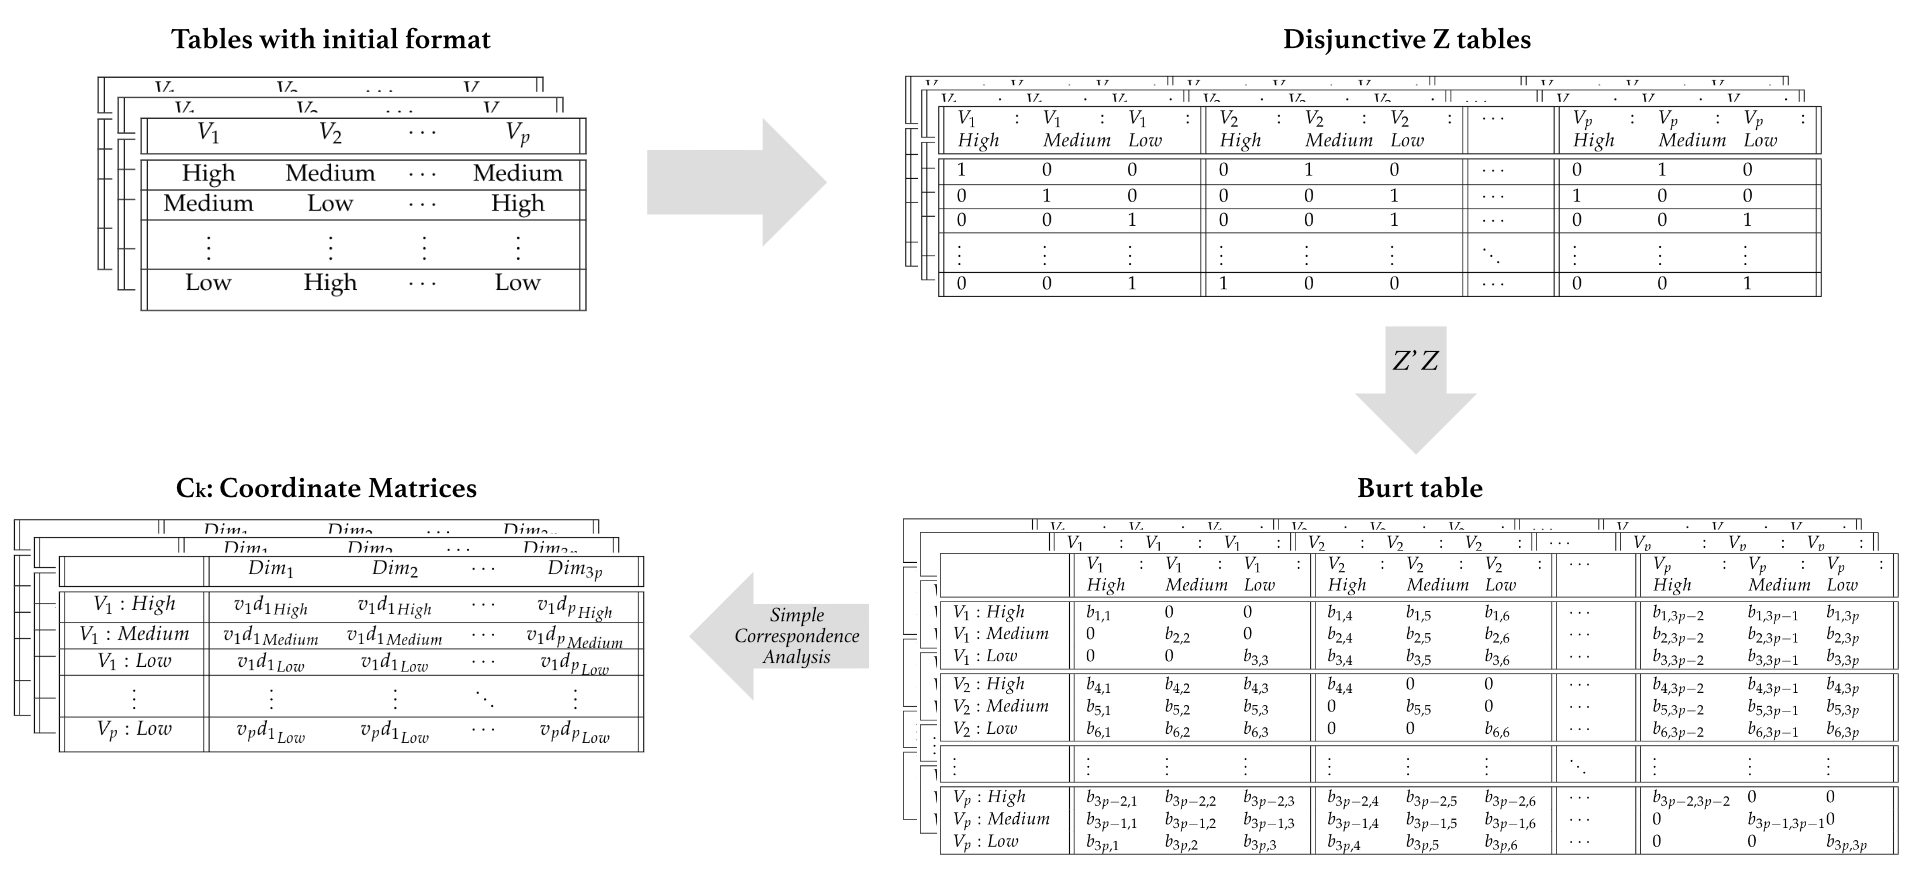
\includegraphics[width=0.9\linewidth,]{ktablesMCAi} \end{center}

\caption{Procedure of MCA for $K$ tables}

\label{fig:MCAk}
\end{figure}

Each of the \(K\) sets of coordinates obtained in the previous step is
denoted as \(C\). In order to detect the magnitude of the latent
variables, the absolute value of the elements of the matrix
\(C_{k} (k=1,…, K)\) is taken. Thus, a set of \(K\) tables of
coordinates (loadings) is obtained, whose rows correspond to the
observed variables and the columns to the latent variables.

\hypertarget{normalization-of-tables}{%
\subsubsection{Normalization of tables}\label{normalization-of-tables}}

Normalization \citep{AFM} from Multiple Factor Analysis (MFA) is applied
to the \(K\) tables \textbf{C}.

Let \(\lambda_{1}^{k}\) be the first eigenvalue obtained from the
singular value decomposition of the \(k\)-th table \textbf{C}. The table
is normalized by multiplying it by \(1/\lambda_{1}^{k}\). This results
in the table \(C^{'}\), which corresponds to the normalized coordinate
table. Individually, for the case of the \(k\) matrix, the following
expression would be obtained.

\begin{equation}
\mathbf{C'_k}=\frac{1}{\lambda_{k}^1} \mathbf{C_k}
\label{eq:Cprimak}
\end{equation}

Up to this point, we have a set of normalized coordinate matrices, whose
rows contain the observed variables and columns contain the latent
variables.

The expression in equation \ref{eq:Cprimak} applied to \emph{K} tables
is represented in Figure \ref{fig:esquema1}, which shows the scheme for
preparing the tables prior to obtaining centrality vectors used by the
multivariate control chart.

\begin{figure}[!ht]


\begin{center}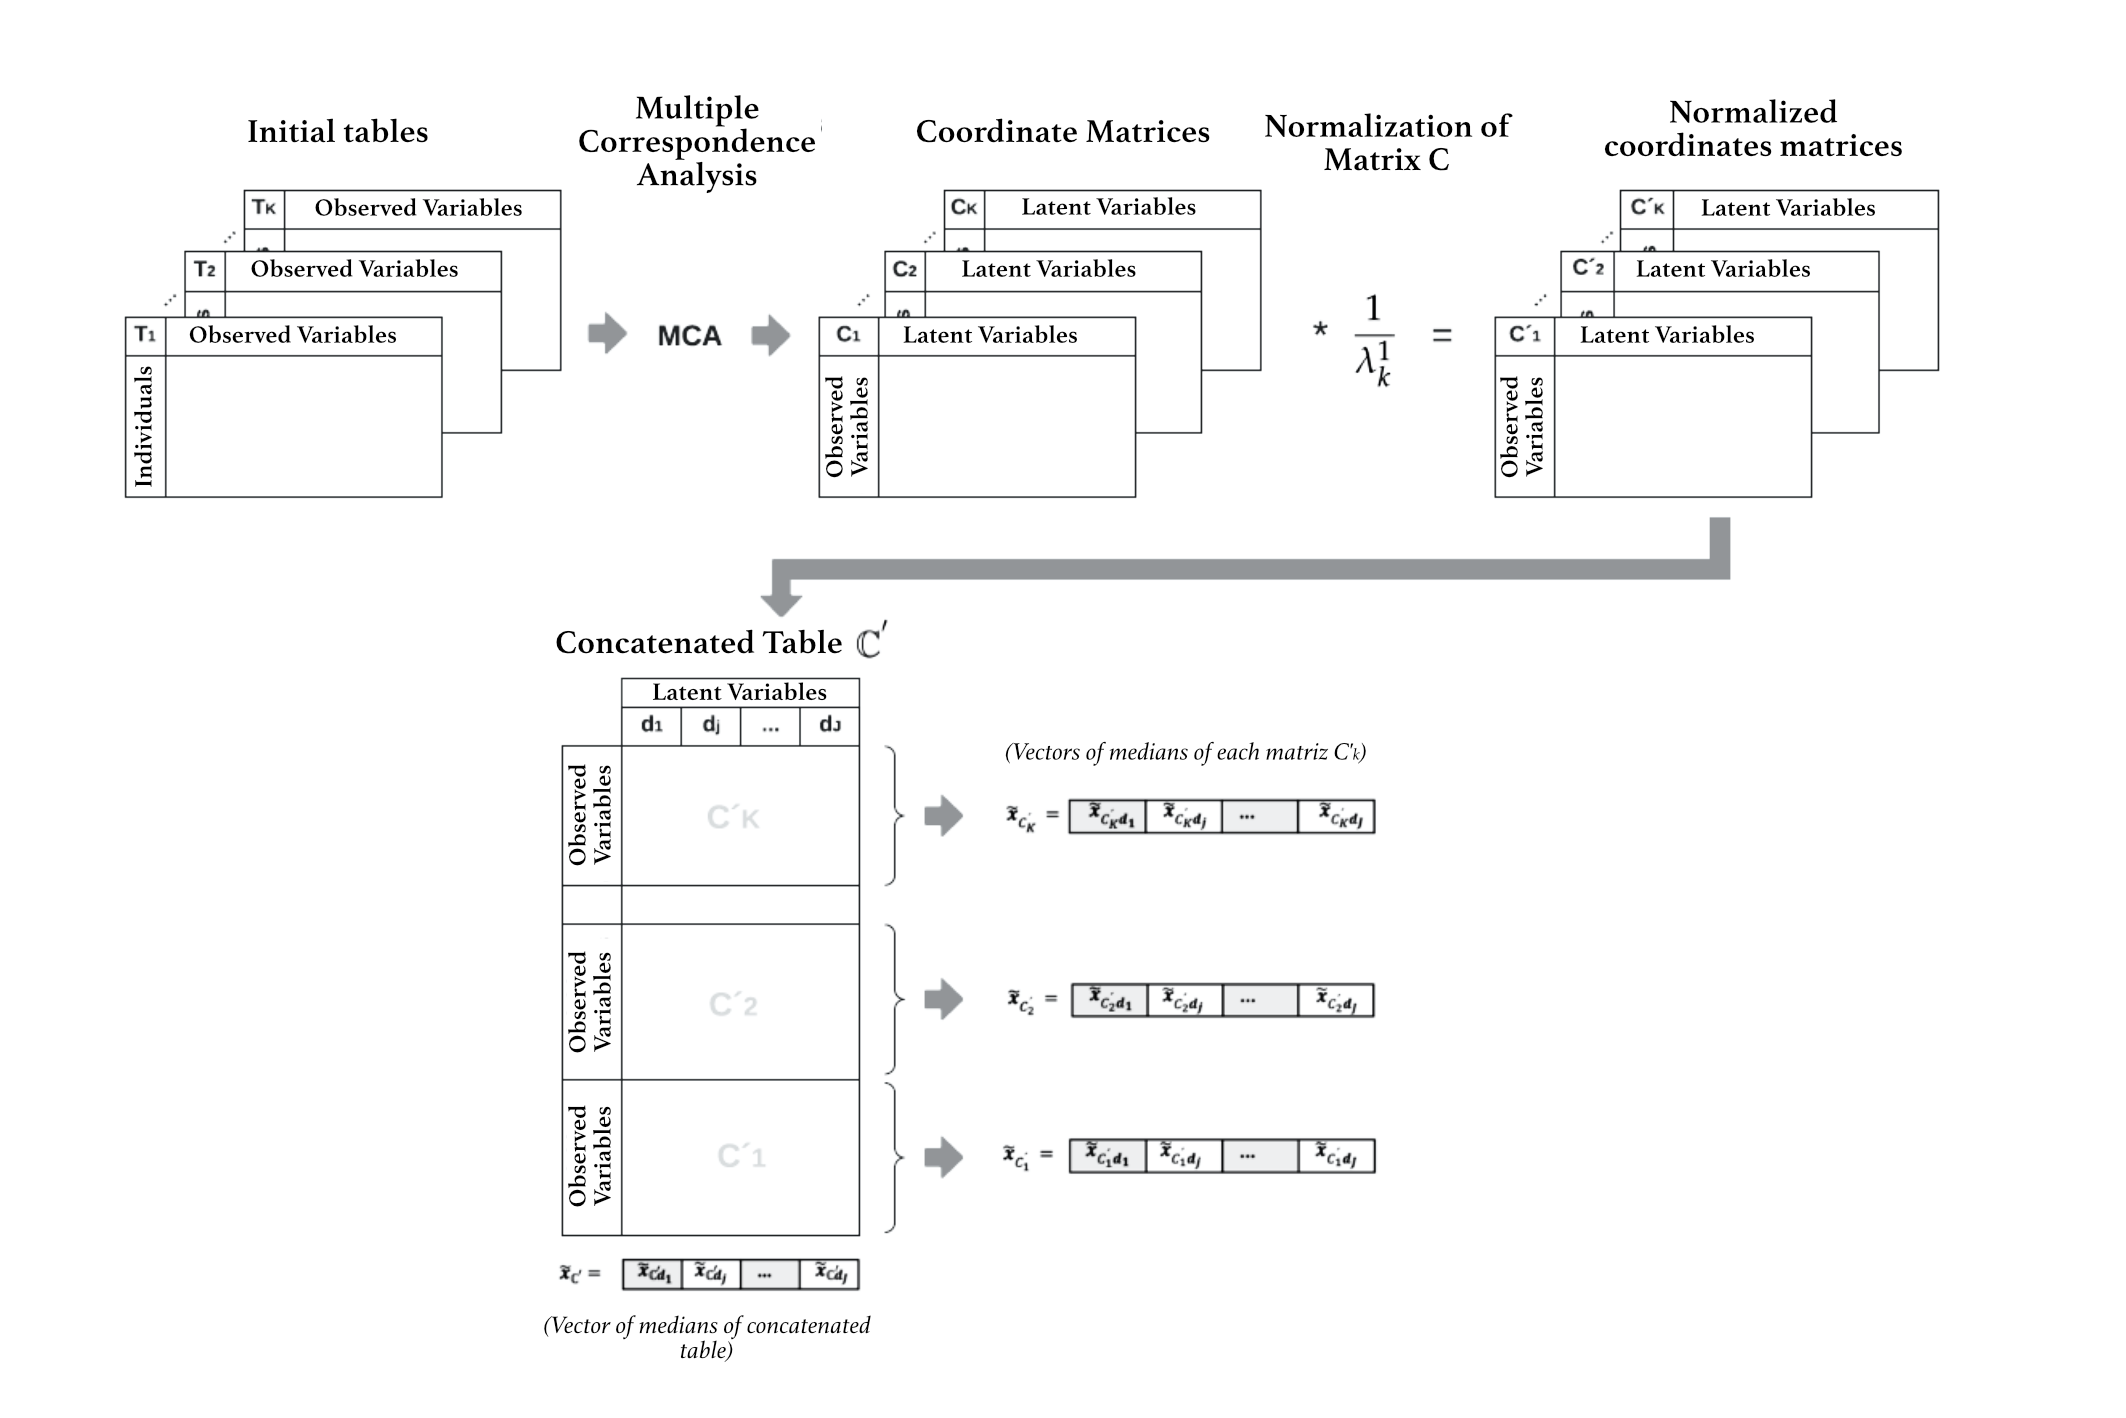
\includegraphics[width=0.9\linewidth,]{esquema_1i} \end{center}

\caption{Scheme of the process for obtaining median vectors}

\label{fig:esquema1}
\end{figure}

By unifying the \emph{K} normalized tables \(C^{'}\) into a single one,
we obtain the concatenated matrix \(\mathbb{C}^{'}\), which contains all
the elements of the \emph{K} normalized tables.

\begin{equation}
\mathbf{\mathbb{C^{'}}}=[\mathbf{C_1^{'}}|\mathbf{C_2^{'}}|,...,|\mathbf{C'_{K}}]^{T}
\label{eq:Cprima}
\end{equation}

The normalization performed by MFA is responsible for weighting the
\emph{K} tables, with the aim of avoiding any imbalance when carrying
out the joint analysis of the tables.

From the matrices \(\mathbf{\mathbb{C^{'}}}\) and \(\mathbf{C_k^{'}}\),
the median vectors are obtained, as shown in Figure \ref{fig:esquema1}.

The vector \(\mathbf{\tilde{x}_{C_k^{'}}}\) explains the central
behavior of table \emph{k}, and the vector
\(\mathbf{\tilde{x}_{\mathbb{C^{'}}}}\) explains the behavior of the
concatenated matrix.

\hypertarget{t2qv-control-chart}{%
\subsection{T2Qv Control Chart}\label{t2qv-control-chart}}

\hypertarget{obtaining-the-control-chart}{%
\subsubsection{Obtaining the control
chart}\label{obtaining-the-control-chart}}

To define the Hotelling \(T^2\) control chart, the following
considerations must be taken into account:

\begin{itemize}
\tightlist
\item
  The matrix \(\mathbb{C}^{'}\) (Equation \ref{eq:Cprima}) is called
  Concatenated and serves as a reference for the in-control scenario in
  phase I of the process control.
\item
  The Hotelling \(T^2\) statistic is usually calculated with the mean
  vectors and covariance matrix of the in-control process. The proposal
  of this research is to adopt robustness concepts, using the median
  vector instead of the mean vector, because medians are not affected by
  outliers.
\item
  From the concatenated matrix \(\mathbb{C}^{'}\), we obtain
  \(\tilde{x_{0}}\) (median vector of the concatenated matrix) and
  \(S_0\) (covariance matrix of the concatenated matrix).
\item
  Each matrix \(\mathbf{C'_k}\) has the same number of columns.
\item
  The mean vector \(\tilde{x_{k}}\) is tied to the table
  \(\mathbf{C'_k}\), meaning that the control chart will depend on the
  differences between the matrices \(\mathbf{C'_k}\) and the
  concatenated matrix \(\mathbf{\mathbb{C^{'}}}\).
\item
  The matrices \(\mathbf{C'k}\) follow a multivariate normal
  distribution with median vector \(\tilde{x_{k}}\) and covariance
  matrix \(\mathbf{S_k}\).
\end{itemize}

The statistic \(T^2\) is given by:

\begin{equation}
T^2=n (\mu_{k}-\mu_{0})'\mathbf{\Sigma_{0}^{-1}}(\mu_{k}-\mu_{0})
\label{eq:T2}
\end{equation}

Taking into account the aforementioned considerations, the statistic
\(T^2_{med}\) is obtained.

\begin{equation}
T^2_{med}=n (\tilde{x_{k}}-\tilde{x_{0}})'\mathbf{\Sigma_{0}^{-1}}(\tilde{x_{k}}-\tilde{x_{0}})
\label{eq:T2med}
\end{equation}

It is known that, under control, \(T^2\) is distributed as a Chi-squared
with \(p\) degrees of freedom, \(\chi^2_p\). In this case, this
principle can be applied, as the Concatenated matrix
(\(\mathbb{C}^{'}\)) is used, which represents the in-control scenario.

Since this control chart is based on weighted Mahalanobis distances, it
only has an upper control limit. This is given by Equation \ref{eq:UCL}.

\begin{equation}
UCL=\chi^2_{\alpha,p}
\label{eq:UCL}
\end{equation}

where \(p\) is the number of dimensions and \(\alpha\) is the
predetermined significance level, with \(\alpha=0.0027\) being
considered.

\begin{figure}[!h]


\begin{center}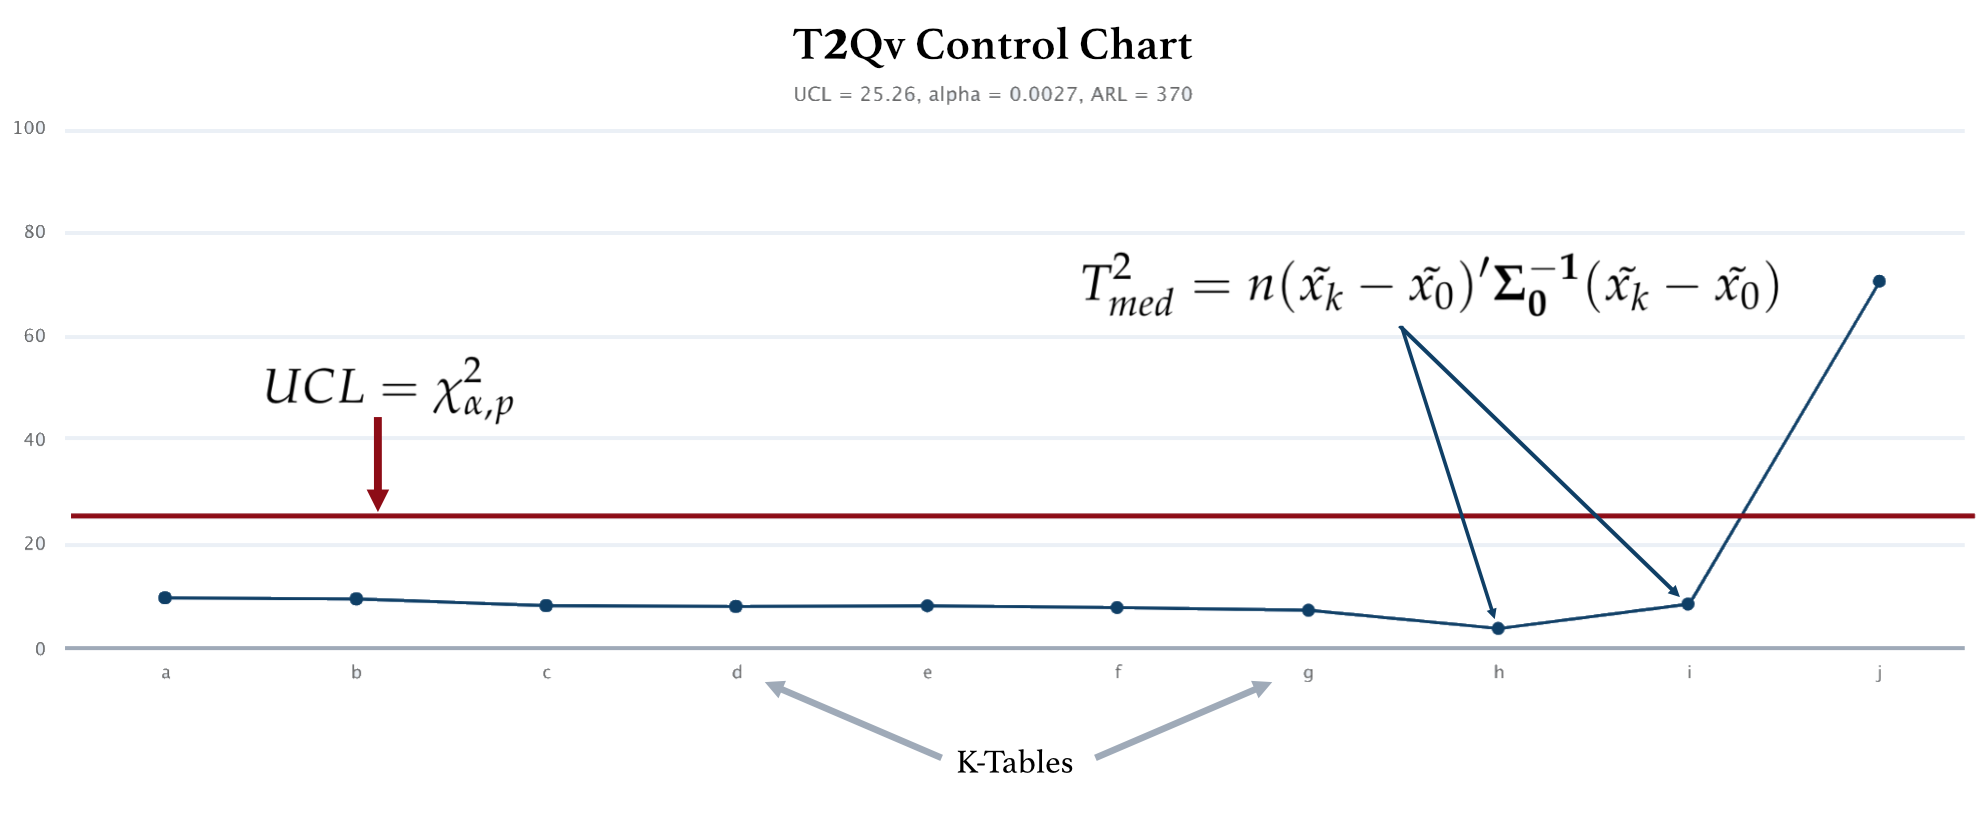
\includegraphics[width=0.7\linewidth,]{t2qvesqi} \end{center}

\caption{T2Qv Control Chart}

\label{fig:t2qvesq}
\end{figure}

\hypertarget{interpretation-of-out-of-control-points}{%
\subsubsection{Interpretation of out-of-control
points}\label{interpretation-of-out-of-control-points}}

The multivariate chart for qualitative variables, T2Qv, is capable of
indicating that the process has gone out of control, but it does not
allow recognizing the causes for this to happen. Each point represented
on the chart represents a table (sample), consisting of a group of
individuals (observations) and \emph{p} variables that can have many
categories, some of which may exhibit anomalous behavior. Therefore, it
is necessary to carefully analyze what is happening with the data of the
reported tables to identify the variable(s) that caused the process to
go out of control.

This analysis is performed by comparing the location of the points
representing the categories of the variables in the MCA of the
concatenated table and the location of the points in the MCA charts of
each table reported as out of control. The categories that are
influencing the out-of-control state are those that show noticeable
differences in their location when comparing both tables. To quantify
the magnitude of these differences or the anomalous behavior of these
categories, the Chi-squared distances between the masses of the columns
of the table reported as out of control and the columns of the
concatenated table, taken as a reference, are calculated. The higher the
value of the statistic, the greater its incidence in the displacement of
the centrality of the process that can ultimately lead to an
out-of-control state.

\hypertarget{computational-complement}{%
\section{Computational complement}\label{computational-complement}}

To facilitate the dissemination and application of the proposed method,
a reproducible package has been developed in R. The \textbf{T2Qv}
package \citep{T2Qv} performs the analysis of control of \emph{K} tables
through multivariate control charts for qualitative variables, using the
theoretical foundations of multiple correspondence analysis and multiple
factor analysis, as well as the conceptual idea of STATIS.

The charts can be displayed in flat or interactive form, and all outputs
can be shown in an interactive Shiny panel, and their graphical and
numerical results can be exported.

\hypertarget{description-of-the-t2qv-package}{%
\subsection{Description of the T2Qv
package}\label{description-of-the-t2qv-package}}

The statistical package T2Qv performs Multiple Correspondence Analysis
on the original tables (\(\mathbf{T_k}\)), generating latent variable
matrices (\(\mathbf{C_k}\)) whose coordinates are subjected to a
normalization process, multiplying them by \(1/\lambda_{1}^{k}\). The
normalized coordinate matrices (\(\mathbf{T'_k}\)) are ordered one below
the other, to form a concatenated table (\(\mathbb{C}^{'}\)), from which
the median vector \(\tilde{\tilde{\mathbf{x}}}_{\mathbb{C'}}\) is
extracted, as well as the median vectors of each matrix
\(\tilde{\tilde{\mathbf{x}}}_{\mathbf{C'{k}}}\)) that conform it.

With these vectors, the statistics
\(T^2_{med}=n (\tilde{x_{k}}-\tilde{x_{0}})'\mathbf{\Sigma_{0}^{-1}}(\tilde{x_{k}}-\tilde{x_{0}})\)
are obtained for each of the analyzed tables, which are represented as
points in the T2Qv control chart. Points that fall outside the limit
(\(UCL= \chi_{\alpha,p}^2\)) are reported as out of control.

The T2Qv statistical package allows the interpretation of the anomalous
behavior of points outside of control through the comparison of the MCA
charts of a table \(\mathbf{TC_k}\), which results from concatenating
the initial matrices, and each initial table \(\mathbf{T'_k}\). The
package allows for the selection of the \(\mathbf{T'_k}\) tables, so
that the researcher can focus their analysis on those identified as out
of control.

In addition, the T2Qv package generates an interactive bar chart that
represents the \(\chi^2\) distances between the column masses of the
variables in the \(\mathbf{TC_k}\) table and the \(\mathbf{T'_k}\)
table. Bars denoting greater height identify the variables that are most
strongly causing the out-of-control output of the \(k\)-th table. This
interactive chart includes, through a nested circular chart, a
representation of the distribution of the observed variable categories
corresponding to the \(k\)-th table, as well as a circular chart of the
distribution of categories in the concatenated table
(\(\mathbf{TC_k}\)), facilitating the identification of changes in
category distribution.

Thus, the T2Qv package consolidates the methodology proposed in this
research and allows for an explanation of when and why the process went
out of control.

The functions included in the package and their description are listed
in Table \ref{tab:functions}.

\begin{table}[h!]
\begin{center}
 \begin{tabular}{||c  m{35em}||} 
 \hline
  Function & Description \\ [0.5ex] 
 \hline\hline
 T2 qualitative & Multivariate control chart T2 Hotelling applicable for qualitative variables.\\
 \hline
  MCAconcatenated & Multiple correspondence analysis applied to a concatenated table.\\
\hline
  MCApoint & Multiple correspondence analysis applied to a specific table.\\
\hline
  ChiSq variable & Contains Chi square distance between the column masses of the table specified in PointTable and the concatenated table. It allows to identify which mode is responsible for the anomaly in the table in which it is located. \\ [1ex] 
  \hline
  Full Panel & A shiny panel complete with the 
  multivariate control chart for 
  qualitative variables, the two MCA 
  charts and the modality distance table. 
  Within the dashboard, arguments such as 
  type I error and dimensionality can be 
  modified. \\ [1ex] 
 \hline
\end{tabular}\caption{Functions of the T2Qv package}
\label{tab:functions}
\end{center}
\end{table}

\hypertarget{availability}{%
\subsection{Availability}\label{availability}}

The package is available on the official R repository, The Comprehensive
R Archive Network (CRAN), and can be downloaded as follows:

\begin{verbatim}
install.packages("T2Qv")
\end{verbatim}

\hypertarget{results}{%
\section{Results}\label{results}}

To test the proposed methodology in the Hotelling's \(T^2\) control
chart for qualitative variables, an analysis was conducted using
simulated data and another using real data applied in the context of
higher education. The results were obtained through the application of
the T2Qv package.

\hypertarget{results-with-simulated-data}{%
\subsection{Results with simulated
data}\label{results-with-simulated-data}}

\hypertarget{simulated-data-generation}{%
\subsubsection{Simulated data
generation}\label{simulated-data-generation}}

\label{simulados}

For this study, a simulated database was generated, called
\emph{Datak10Contaminated.} It consists of 10 tables, each one composed
of 100 rows (observations) and 11 columns, of which the first 10
correspond to the analyzed variables (V1, V2, \ldots, V10), which
contain 3 categories (High, Medium, and Low), while column 11, called
\emph{GroupLetter}, contains the classification factor of the groups.
For their identification, the tables have been named with the letters of
the alphabet, from \emph{a} to \emph{j.} Table \emph{j} has a different
distribution than the other nine.

The first 9 tables have their 10 variables with the following
distribution:

\[ u \sim U[0,1]\]

\[t_{1,..,9}= \left\{ \begin{array}{lcc}
             Low &   si  & u \leq 1/3 \\
             \\ Medium &  si & 1/3 < u < 2/3 \\
             \\ High &  si  & u \geq 2/3 
             \end{array}
   \right. \]

Table \emph{j} or Table 10, in all its 10 variables, follows the
distribution presented below:

\[ u \sim U[0,1]\]

\[t_{j}= \left\{ \begin{array}{lcc}
             Low &   si  & u \leq 1/5 \\
             \\ Medium &  si & 1/5 < u < 2/6 \\
             \\ High &  si  & u \geq 2/6 
             \end{array}
   \right. \]

The database is presented in the format established in table
\ref{tab:tabladatos}.

\begin{table}[!ht]
\tiny
\centering
\resizebox{13cm}{!} {
\begin{tabular}{@{}lllllllllll@{}}
\toprule
\textbf{V1}                  & \textbf{V2}                    & \textbf{V3}                  & \textbf{V4}                    & \textbf{V5}                  & \textbf{V6}                    & \textbf{V7}                    & \textbf{V8}                    & \textbf{V9}                    & \textbf{V10}                   & \textbf{GroupLetter}      \\ \midrule
Low      & Medium     & Medium                       & High                           & High                         & High                           & Low                            & Medium                         & Medium                         & Medium                         & a                         \\
Low                          & Low                            & High                         & Low                            & Medium                       & High                           & High                           & High                           & Low                            & High                           & a \\
High & Medium & High & Low    & High & Medium & Medium & High   & Medium & Low    & a                         \\
Medium                       & Medium                         & Low                          & High                           & Low                          & Medium                         & High                           & Low                            & Low                            & High                           & a \\
Low  & Low    & Low  & High   & Low  & High   & High   & High   & Medium & Medium & a                         \\
High                         & High                           & Medium                       & Low                            & High                         & Low                            & Medium                         & Medium                         & High                           & Low                            & a \\
High & High   & Low  & Low    & Low  & Medium & High   & Medium & Medium & High   & a                         \\
Medium                       & Medium                         & High                         & Medium                         & Medium                       & High                           & Medium                         & High                           & High                           & High                           & a \\
Low  & Low    & Low  & Medium & High & Medium & Low    & Medium & Low    & Low    & a                         \\
Medium                       & Medium                         & Medium                       & High                           & Low                          & Medium                         & High                           & Low                            & High                           & Medium                         & a \\ \bottomrule
\end{tabular}
}

\caption{Section of the $Datak10Contaminated$ database.}

\label{tab:tabladatos}

\end{table}

To verify the difference between the distributions of table 10 and the
others, the average of the relative frequencies in the three categories
was calculated from table \emph{a} to \emph{i}, for the 10 variables
(Annex 1). Then, the average of the mean relative frequencies of the 10
variables was calculated. The result allows to compare the distribution
of the categories of the \emph{Datak10Contaminated} table with the
theoretical uniform distribution, as shown in table
\ref{tab:tablapromfreq}.

\begin{table}[H]
\centering
\begin{tabular}{rcp{3cm}p{3cm}}
\hline
\toprule

\textbf{Categories} & \textbf{Uniform theoretical} & \textbf{Mean of the distributions of the variables in the tables $a$, $b$, ...,  $i$} & \textbf{Mean of the distribution of the variables in the table $j$} \\ \midrule
\textbf{High}       & 0.333            & 0.340                & 0.724            \\ 
\textbf{Medium}     & 0.333            & 0.336                & 0.092            \\ 
\textbf{Low}        & 0.333            & 0.324                & 0.184            \\ \midrule
\end{tabular}
\caption{Comparison of the distribution of the categories in the *Datak10Contaminated* table with the theoretical uniform distribution.}
\label{tab:tablapromfreq}
\end{table}

The corresponding goodness-of-fit chi-square tests were applied to
confirm the distribution of the generated data, as well as the
comparison of table \(j\) with the other tables, confirming significant
differences between the distributions (\(p\)-value \(< 0.05\)), as shown
in Appendix 2.

\hypertarget{application-of-t2qv-package-with-simulated-data}{%
\subsubsection{Application of T2Qv package with simulated
data}\label{application-of-t2qv-package-with-simulated-data}}

The first result is the graph of Multiple Correspondence Analysis (MCA)
applied to the concatenated table (Figure \ref{fig:concatenatedfig}).
This table is considered the visual reference for the scenario under
control for the subsequent analysis of tables reported as out-of-control
points in the T2Qv plot.

The MCA reports a total inertia of 63.35\%, dimension 1 representing
53.64\% of the information, while dimension 2 represents 9.71\%. The
points in the graph represent the observations of each of the 10
variables at their three levels: \emph{High}, \emph{Medium}, and
\emph{Low.} In the MCA plot, observations that are located in the center
of the graph represent categories that occur most frequently, while
those furthest from the center are rare cases. In this sense, in the
concatenated table, there are no observations located at the center of
the graph, but they are distributed in groups surrounding the center,
which is explained by the uniform distribution of variable categories in
most of the tables, with no one category predominating.

\begin{figure}[H]


\begin{center}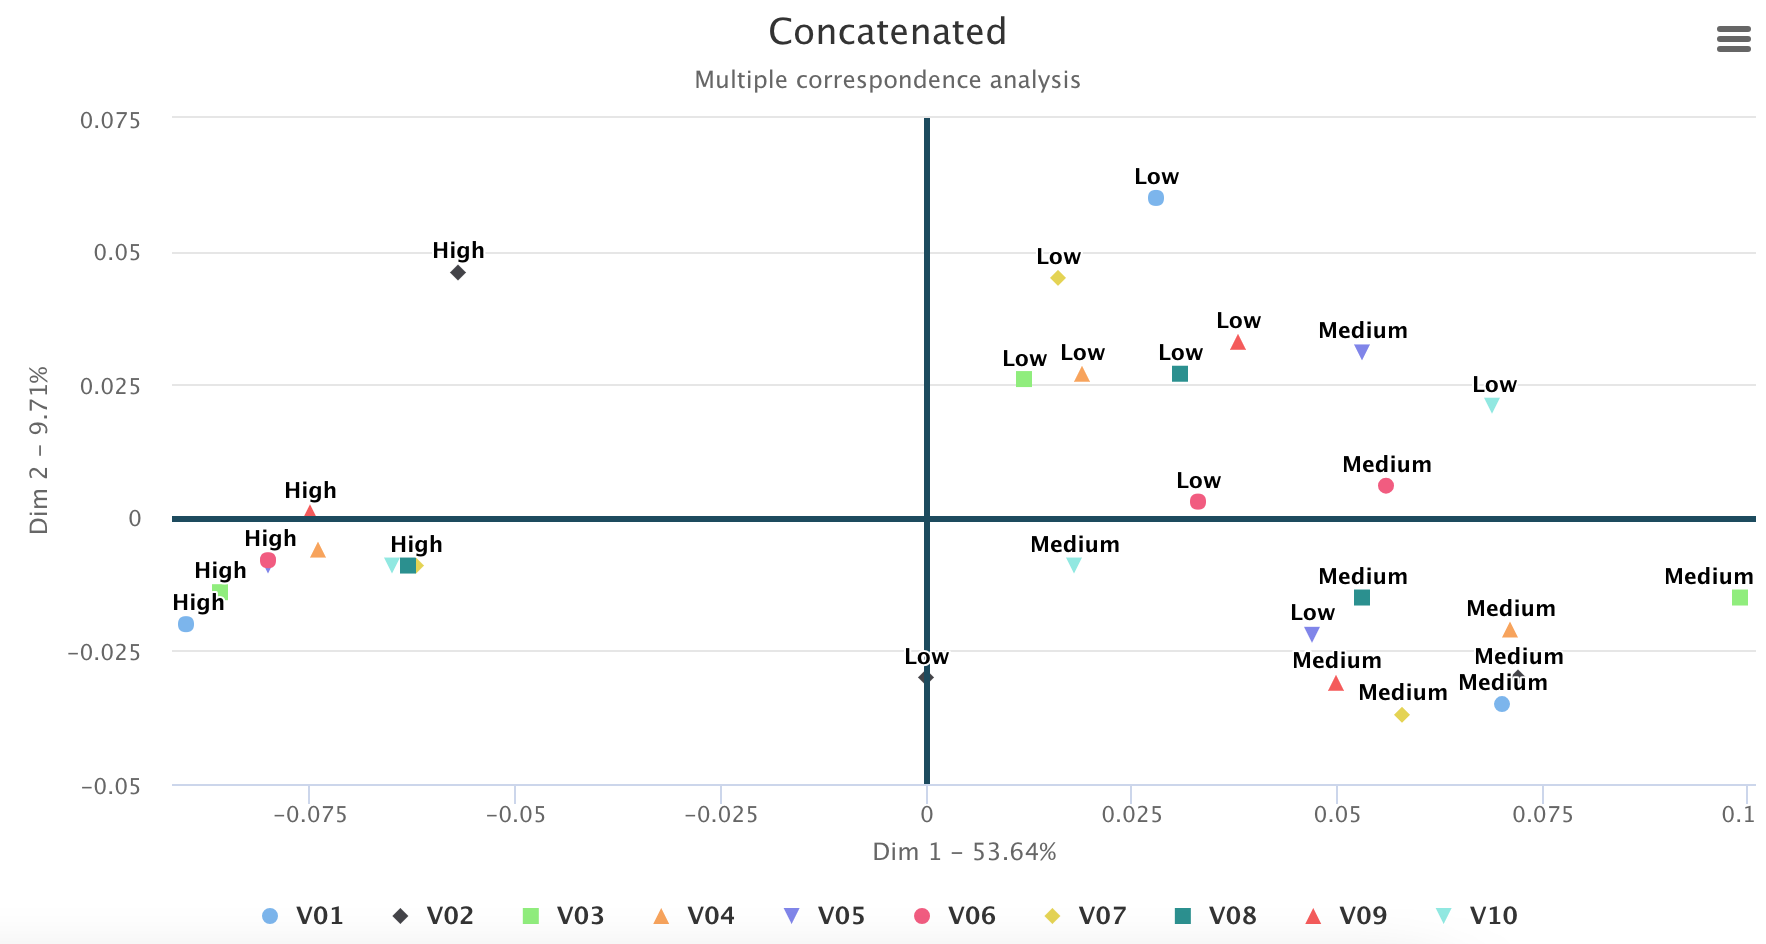
\includegraphics[width=0.9\linewidth,]{concatenated} \end{center}

\caption{Multiple Correspondence Analysis applied to the concatenated table.}

\label{fig:concatenatedfig}
\end{figure}

Another result is the MCA applied to a specific table. At this point,
one of the arguments that must be taken into account is the selection of
the table to be analyzed.

When comparing the plots, it can be observed that the table from point b
(\ref{fig:bfig}) shows differences with the table from the controlled
state (\ref{fig:concatenatedfig}); however, the differences are not
significant enough to generate an out-of-control signal (\ref{fig:tdos},
point b).

\begin{figure}[H]


\begin{center}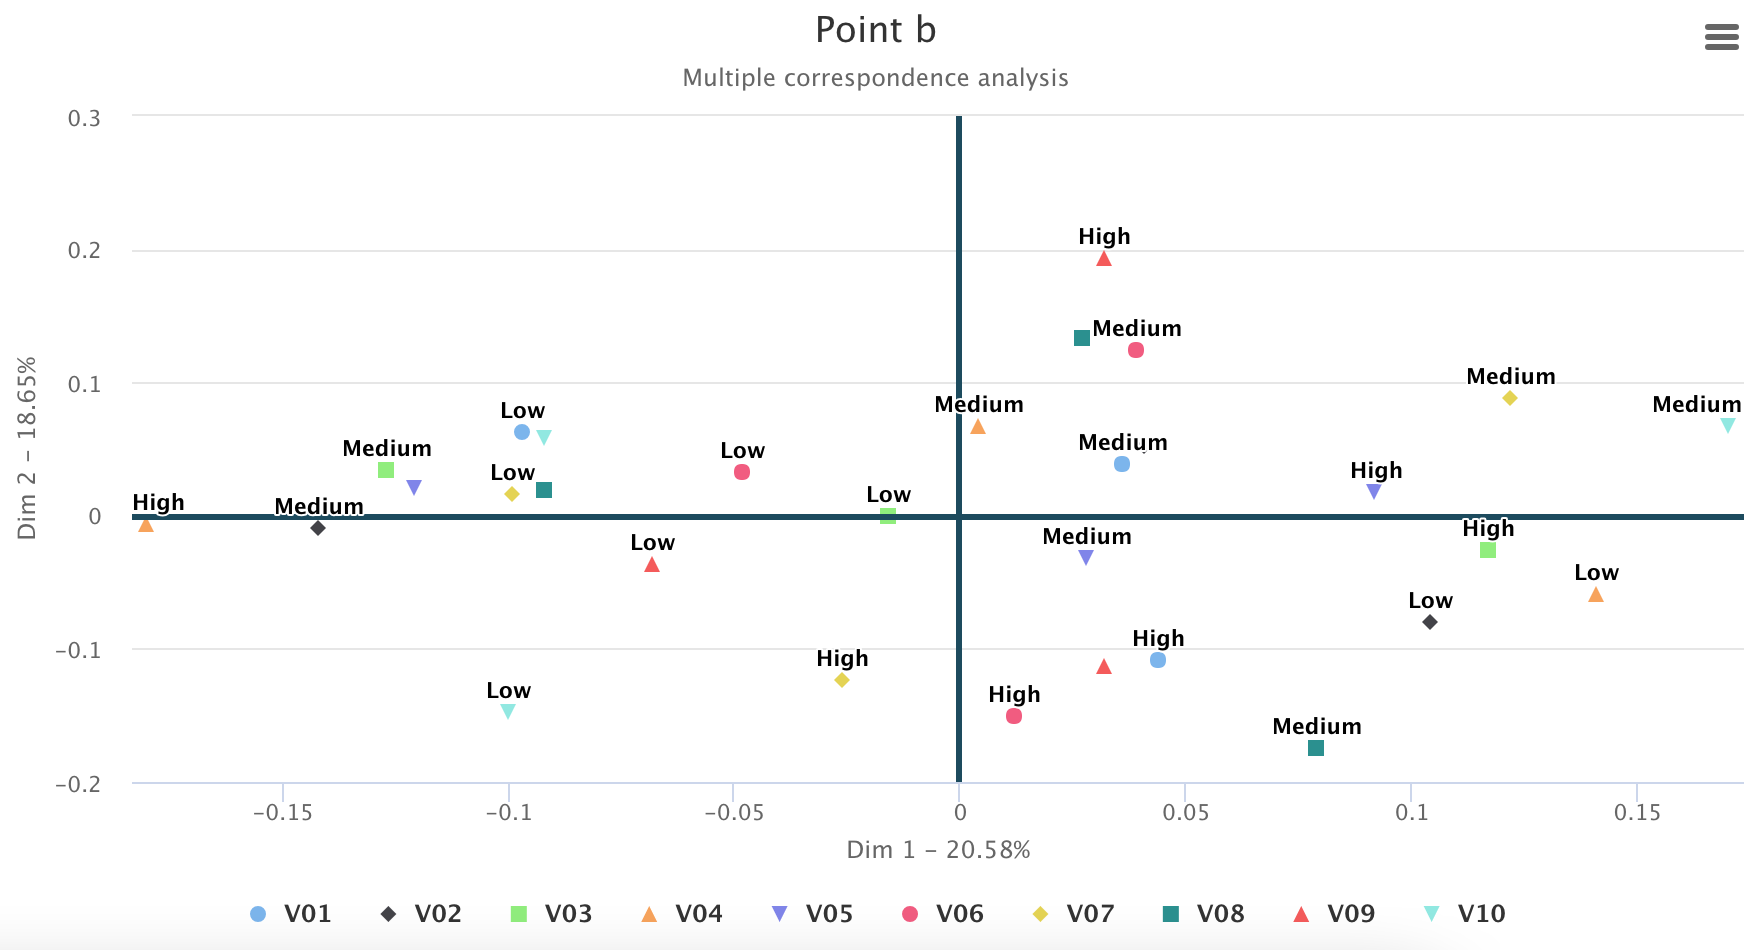
\includegraphics[width=0.9\linewidth,]{pointb} \end{center}

\caption{Multiple Correspondence Analysis applied to Table b.}

\label{fig:bfig}
\end{figure}

The figure \ref{fig:bfig} represents the MCA plot of table b,
corresponding to a specific moment in the monitored process. This plot,
in its two dimensions, represents 39.23\% of the information. It is
noticeable that the observations in their levels \emph{high},
\emph{medium}, and \emph{low} are randomly distributed in all quadrants
of the plot, and a specific pattern of grouping cannot be identified.

The same can be said of the points represented in any of the other
tables because they share the same distribution, except for table j,
which was designed with a different distribution. However, the use of
MCA from figures \ref{fig:bfig} and \ref{fig:concatenatedfig} still does
not allow for detecting whether the process is in control or not. The
identification of out-of-control points can be made through the
graphical representation of the \(T^2_{med}\) statistic, as shown in
figure \ref{fig:tdos}.

\begin{figure}[H]


\begin{center}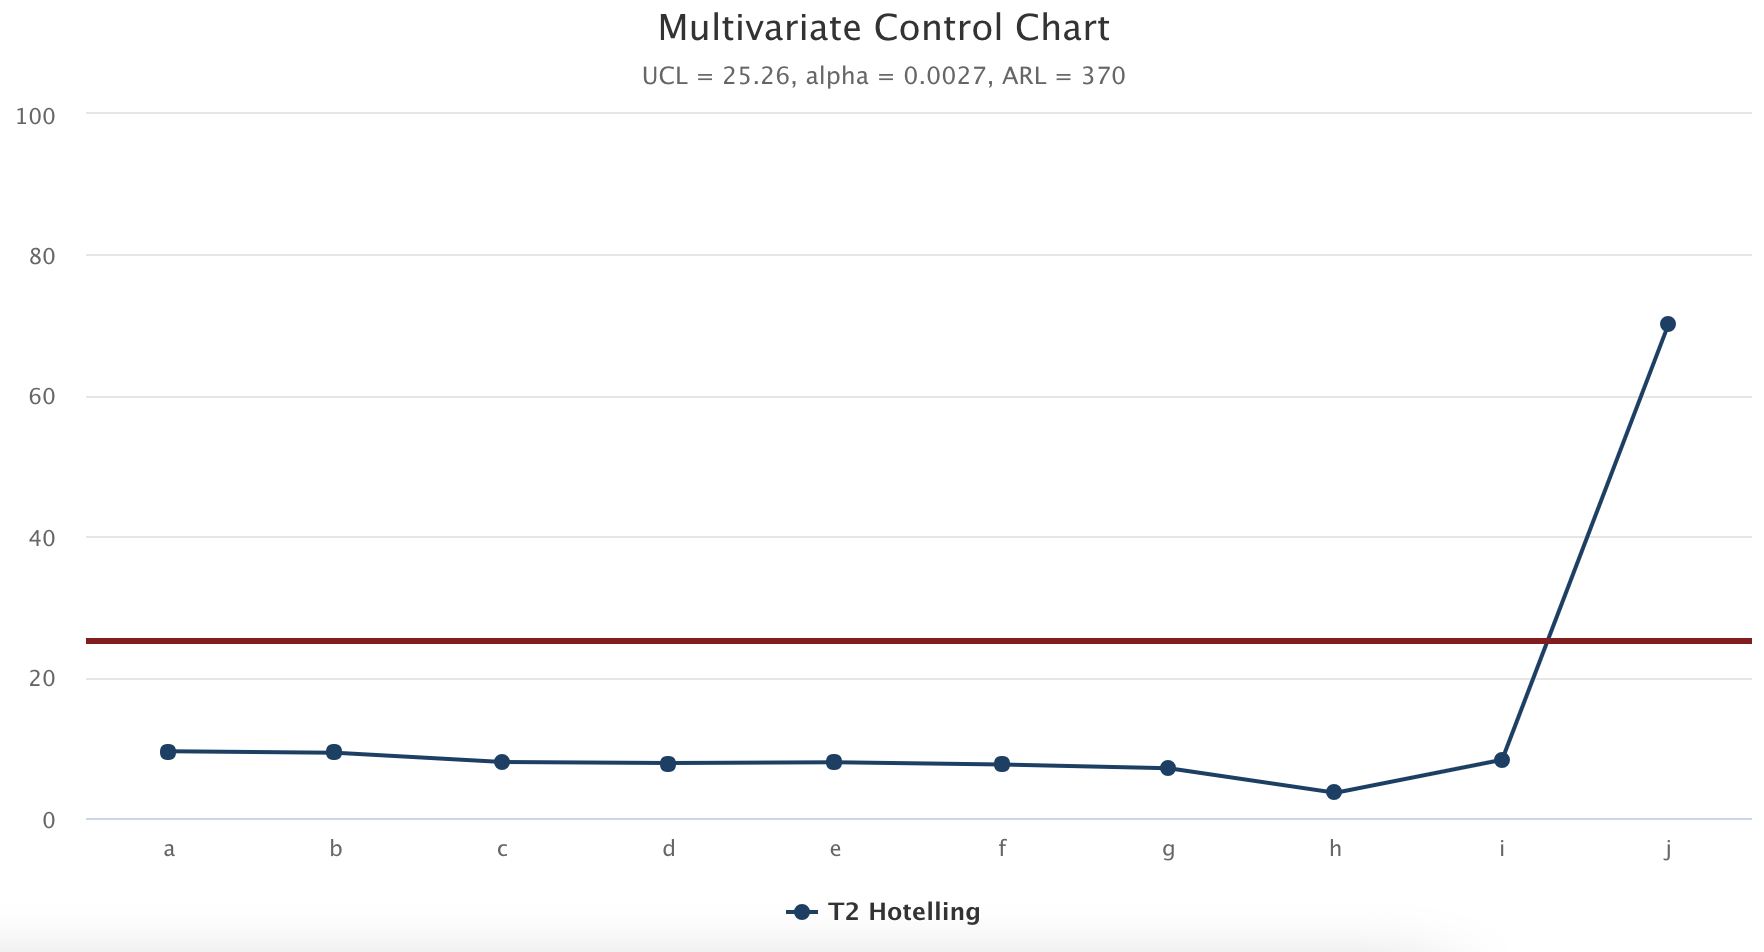
\includegraphics[width=0.9\linewidth,]{t2} \end{center}

\caption{Multivariate control chart T2 Hotelling applied to qualitative variables, $Datak10Contaminated$, figure.}

\label{fig:tdos}
\end{figure}

The figure \ref{fig:tdos} presents the T2Qv control chart, based on the
adjusted Hotelling's T2 statistic (\(T^2_{med}\)), applied to detect
anomalies in any of the \emph{K} analyzed tables. Each of the tables is
represented by the points in the chart. A horizontal line representing
the upper control limit (UCL) is observed. The lower control limit (LCL)
is set to zero.

It is observed that the point representing table j is located above the
upper control limit, meaning it has been identified as an out-of-control
value. Therefore, it is necessary to analyze the reported data of the
table in detail and compare it with the concatenated table to identify
the causes of variation and take appropriate actions. To analyze the
out-of-control point, a MCA plot of table j is generated and compared to
a similar plot of the concatenated table, as presented in figure
\ref{fig:comparation}.

\begin{figure}[H]


\begin{center}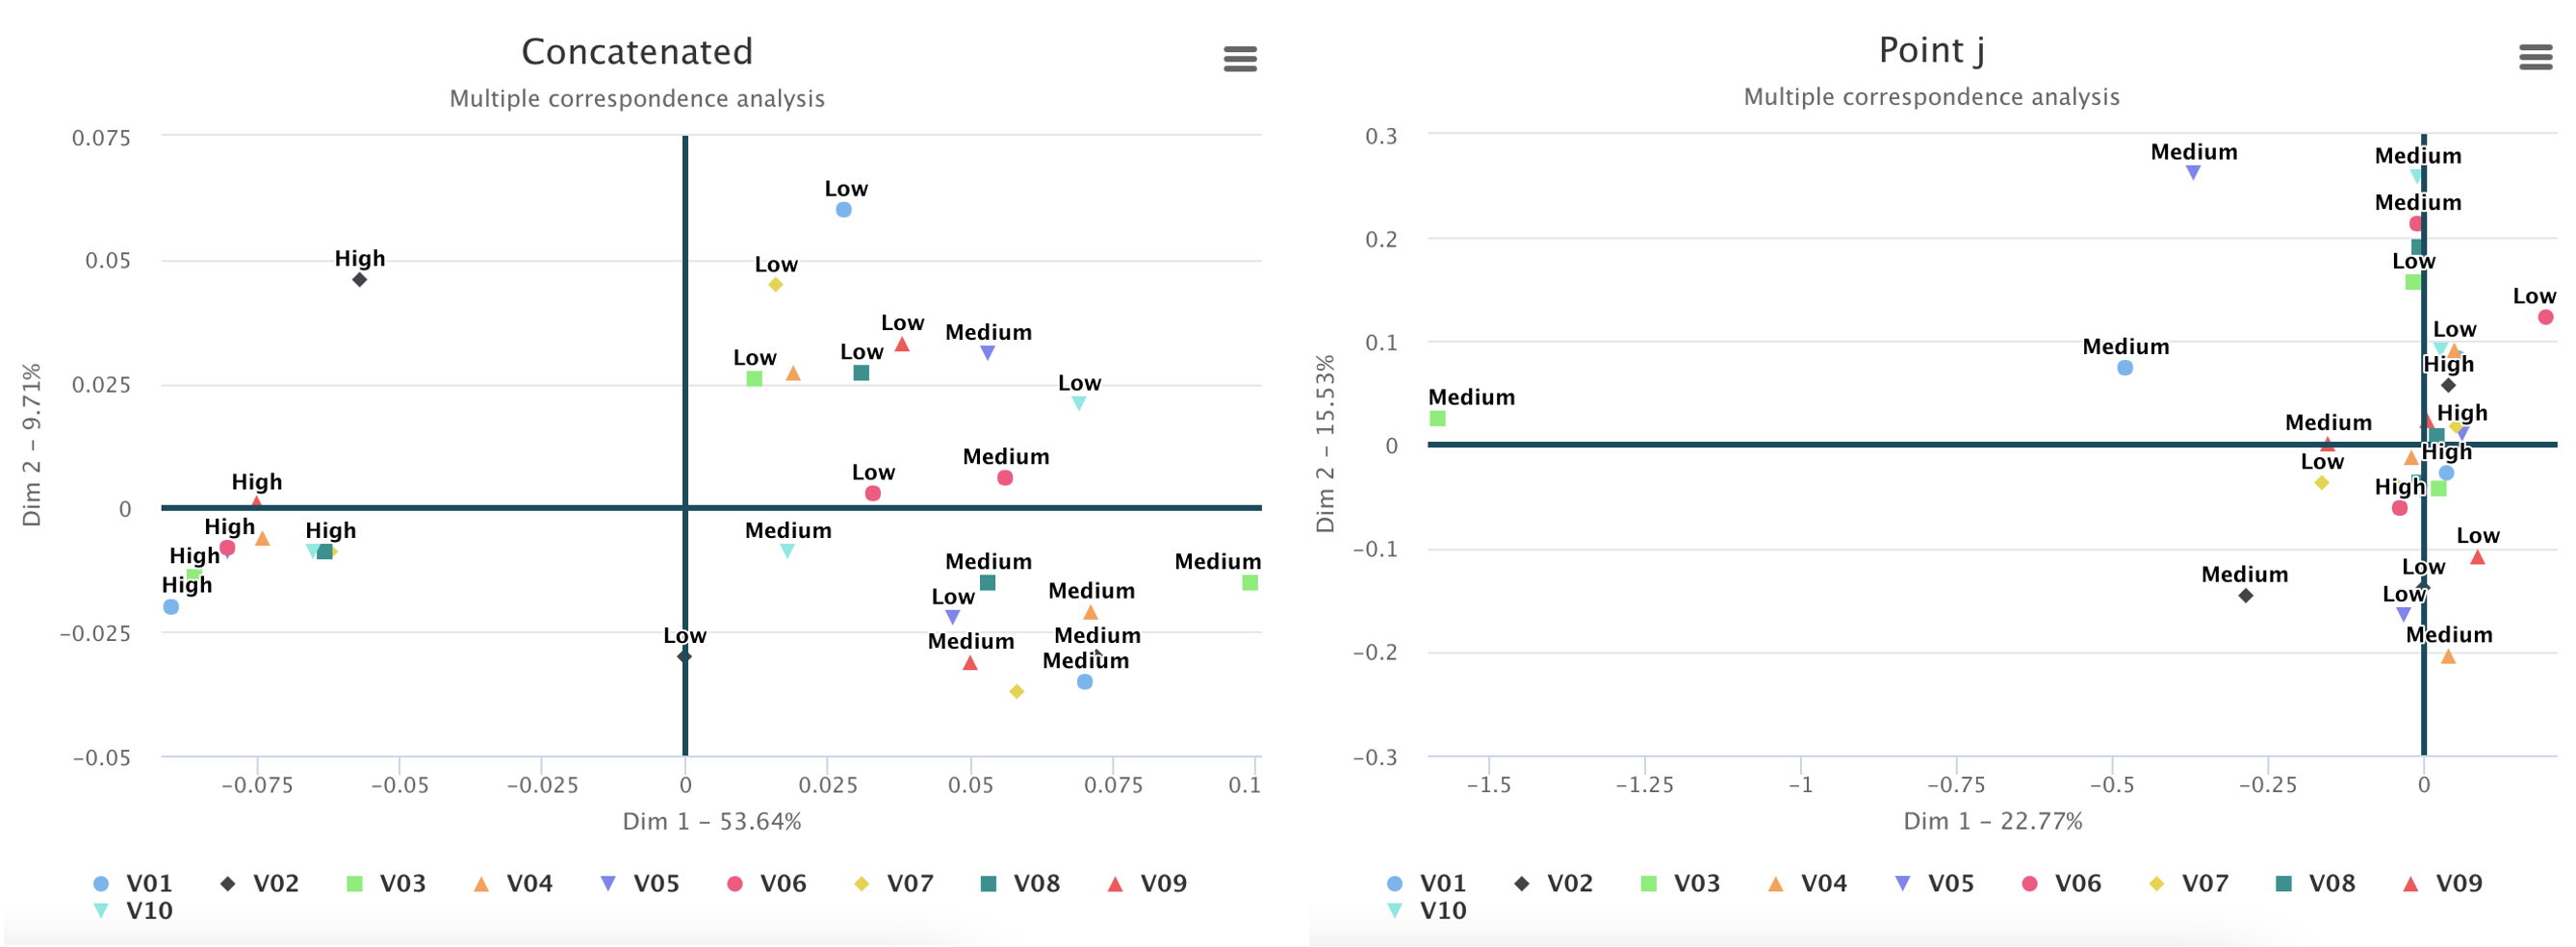
\includegraphics[width=0.9\linewidth,]{comparation} \end{center}

\caption{Multivariate control chart T2 Hotelling applicable to qualitative variables, $Datak10Contaminated$.}

\label{fig:comparation}
\end{figure}

The figure \ref{fig:comparation} presents the distribution of
observations from the concatenated and \emph{j} tables using MCA plots.
The MCA plot of the concatenated table, which serves as the control
reference, was already analyzed in Figure 4. The MCA plot of the
\emph{j} table shows a trend of the mean values of the variables to be
located on the left side, away from the center of the plot, indicating
that the mean values are infrequent. Special attention is deserved by
variable 3, which records an observation for the medium level with the
farthest value from the group. On the contrary, the high categories have
been located at the center, meaning that they are very frequent.

By comparing the plots, it is evident that the data distribution in the
MCA plot of the \emph{j} table is different from the distributions of
the other tables and especially from the data distribution in the MCA
plot of the concatenated table, which explains why the \emph{j} point
was identified as out of control in the T2Qv plot. This difference is
explained in Table 6, which shows the chi-square distance between the
observations of the concatenated table and the \emph{j} table.

\begin{table}[H]
\centering
\begin{tabular}{lr}
\toprule
\multicolumn{1}{c}{\cellcolor[HTML]{FFFFFF}{\color[HTML]{000000} \textbf{Variables}}} & \multicolumn{1}{c}{\textbf{ChiSq}} \\ \midrule

\textbf{V1}                                                                             & {\color[HTML]{333333} 0.06968}      \\ 
\textbf{V2}                                                                       & {\color[HTML]{333333} 0.05010}      \\ 
\textbf{V3}                                                                       & {\color[HTML]{333333} 0.07601}      \\ 
\textbf{V4}                                                                       & {\color[HTML]{333333} 0.04982}      \\ 
\textbf{V5}                                                                       & {\color[HTML]{333333} 0.05205}      \\ 
\textbf{V6}                                                                       & {\color[HTML]{333333} 0.05603}      \\ 
\textbf{V7}                                                                       & {\color[HTML]{333333} 0.03713}      \\ 
\textbf{V8}                                                                       & {\color[HTML]{333333} 0.03702}      \\ 
\textbf{V9}                                                                       & {\color[HTML]{333333} 0.04395}      \\ 
\textbf{V10}                                                                            & {\color[HTML]{333333} 0.06179}      \\ \hline
\end{tabular}
\caption{Chi-square distance between the column masses of table k and the concatenated one, $Datak10Contaminated$.}

\label{tab:chiexamp}
\end{table}

Another way to visualize this information is through a bar chart
generated by the T2Qv application (Figure \ref{fig:chisqr}).

\begin{figure}[H]


\begin{center}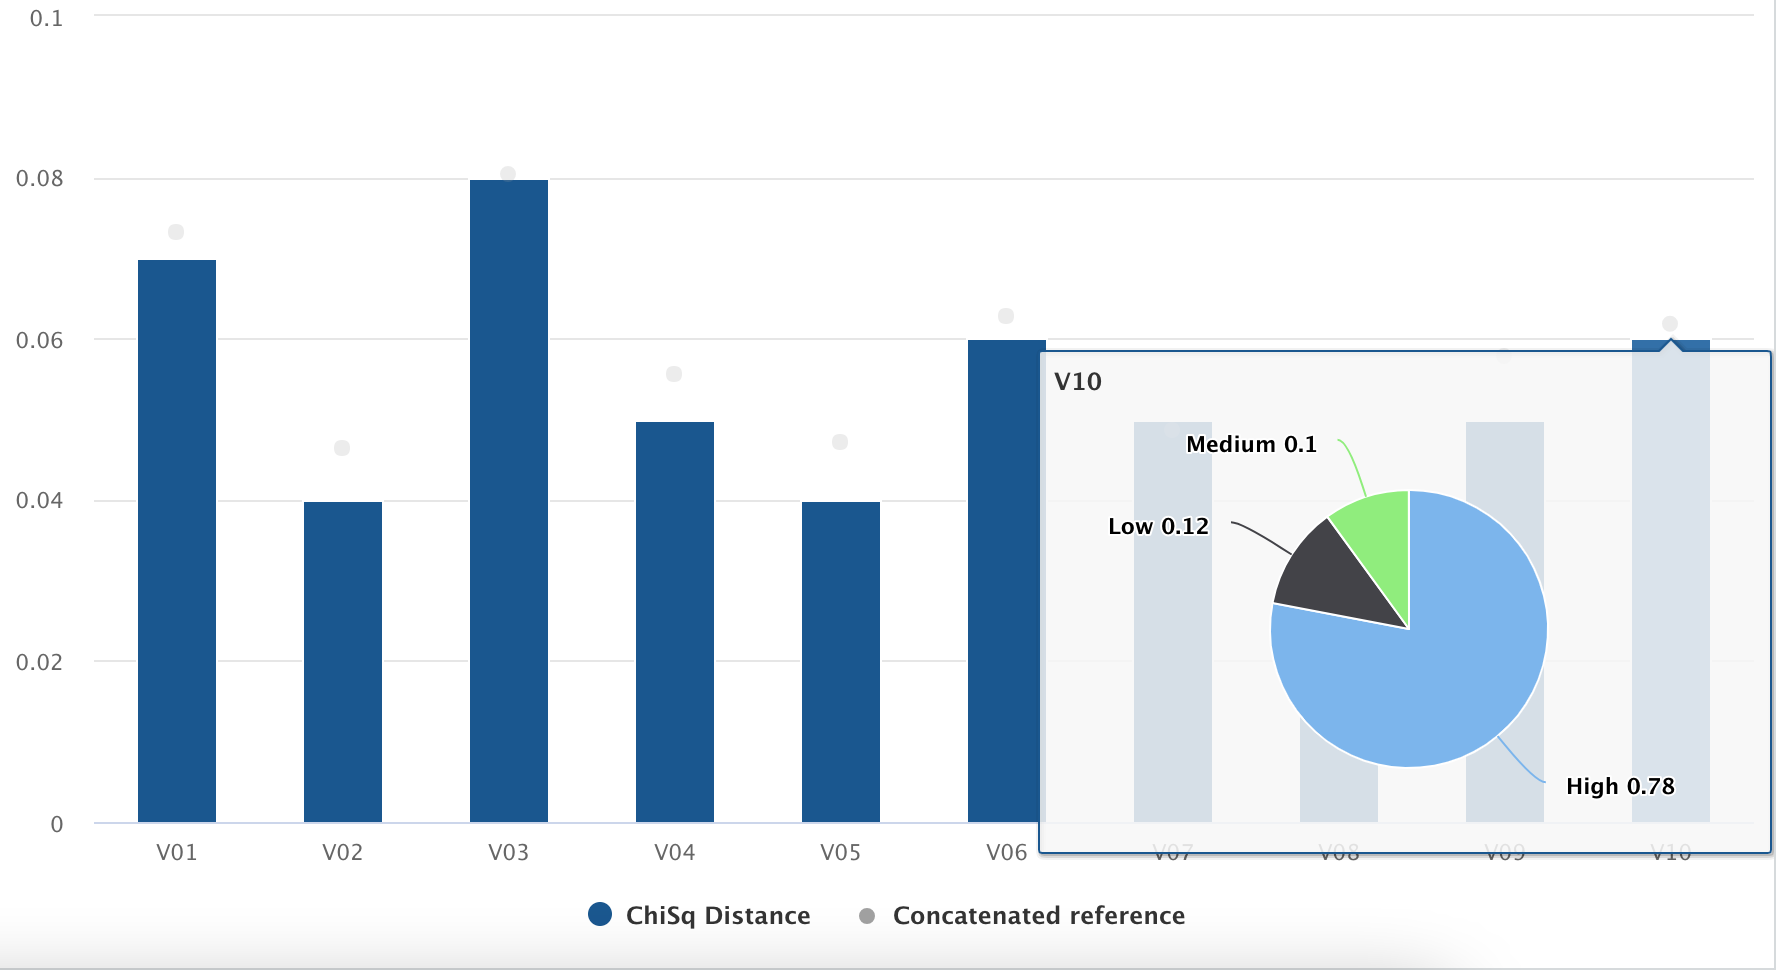
\includegraphics[width=0.9\linewidth,]{Chisqr} \end{center}

\caption{Chi-squared distance between the masses of the concatenated table and the k tables, $Datak10Contaminated$.}

\label{fig:chisqr}
\end{figure}

The bar chart in figure \ref{fig:chisqr} also shows the \(\chi^{2}\)
distance between the masses of the concatenated table and those of the k
tables in the Datak10Contaminated database, in this case table \emph{j}.
Table \ref{tab:chiexamp} shows that variables V03, V01, and V06 exhibit
the highest \(\chi^{2}\) distances between the masses of the
concatenated table and table \emph{j} (0.07700, 0.06968, 0.05938), which
are represented by the tallest bars in figure \ref{fig:chisqr}.

The interactivity of this chart facilitates the observation of the
distribution of the variable categories in the analyzed table, and their
comparison with the distribution of the variable categories in the
concatenated table, as shown in figure \ref{fig:distcomp}.

\begin{figure}[H]


\begin{center}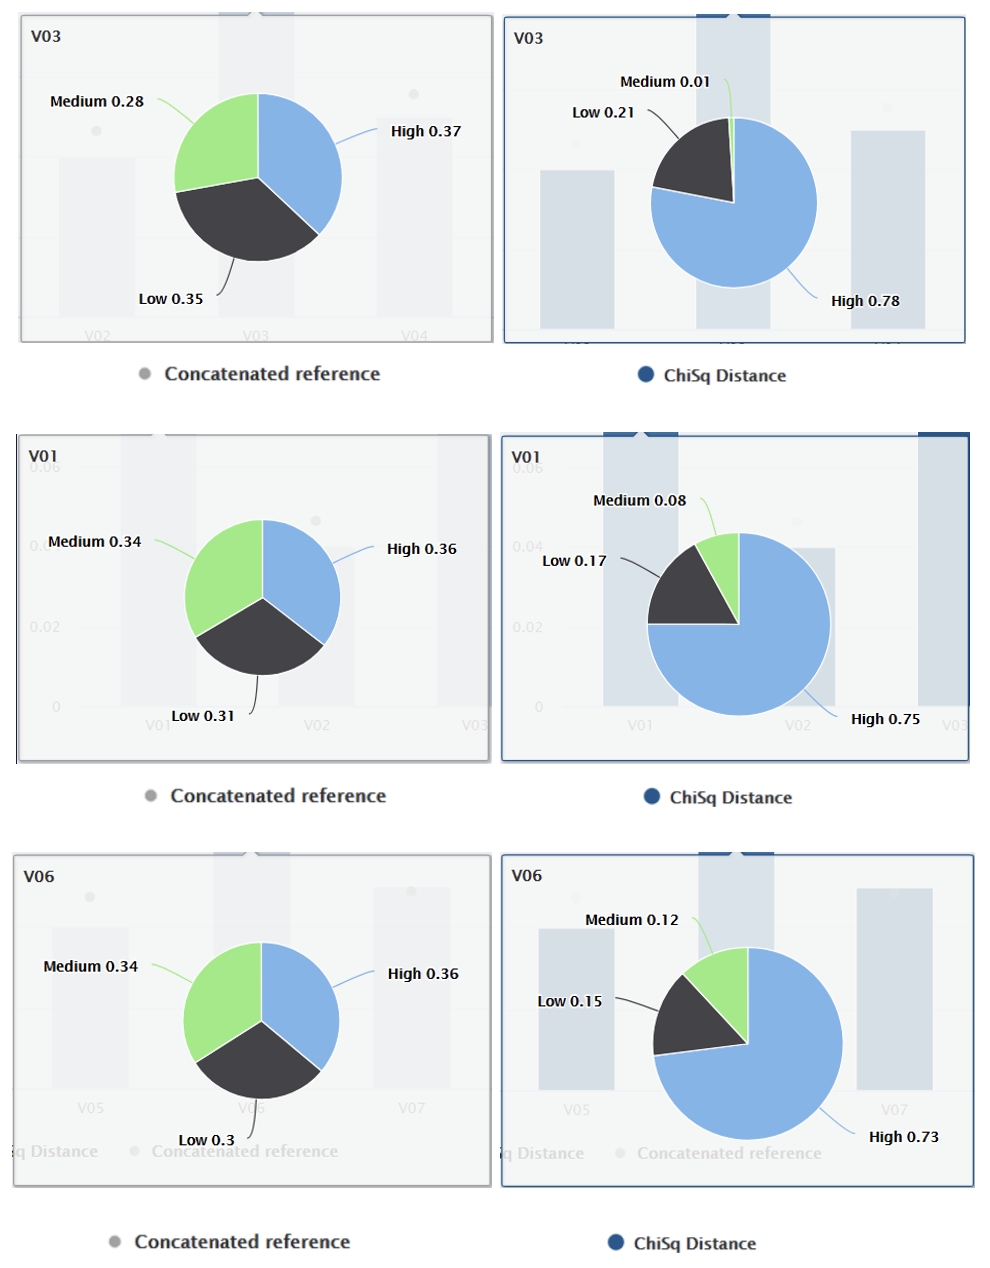
\includegraphics[width=0.9\linewidth,]{distcomp} \end{center}

\caption{Distribution of the categories of variables V03, V01, and V06 in the concatenated table and table $j$ in the T2Qv application.}

\label{fig:distcomp}
\end{figure}

Figure \label{fig:distcomp} presents, in pie charts, the distribution of
categories for variables V03, V01, and V06, which recorded the highest
Chi-squared distances between the masses of the concatenated table and
the \emph{j} table. The charts corresponding to the concatenated table
show sectors with equivalent areas, which is explained by the uniform
distribution of the variables, while those of the \emph{j} table show
areas with varying sizes, where the High category has a relatively high
frequency in all three cases, and Low has a low frequency. Comparing
these charts makes it evident that the distribution of categories
presents significant differences between the concatenated table and the
\emph{j} table.

\hypertarget{sensitivity-analysis}{%
\section{Sensitivity Analysis}\label{sensitivity-analysis}}

As mentioned earlier, in the T2Qv plot, an out-of-control point is
interpreted as a table (\(k_i\)) that includes a quantity or proportion
of contaminated variables. In these cases, it is expected that the
points on the T2Qv plot will generalize the behavior of these
differences in their distribution, thus exceeding the upper control
limit (UCL). The location of this control limit varies depending on the
number of dimensions represented; when it is high, optimal performance
is achieved, while decreasing the number of dimensions that can be
represented introduces instability and reduces the reliability of the
results.

The proposed control chart is capable of detecting an out-of-control
point even with a low number of contaminated variables when working with
a high number of dimensions. It is recommended to use \(p-1\), where
\emph{p} is the total number of dimensions in the initial matrix (Show
in \ref{fig:MCAk}). When the number of dimensions is decreased, the
height of the upper control limit (UCL) also decreases, resulting in an
increased number of out-of-control points, although the variables may
not necessarily express significant differences in their values,
increasing the probability of obtaining a type I error.

Therefore, the question arises as to how many dimensions can be reduced
in the analysis without losing reliability in the result. The importance
of this question lies in the need for a reliable chart that identifies
out-of-control points even if a dimensionality reduction technique has
been applied to the data, without falling into cases of false positives.

\begin{figure}[H]


\begin{center}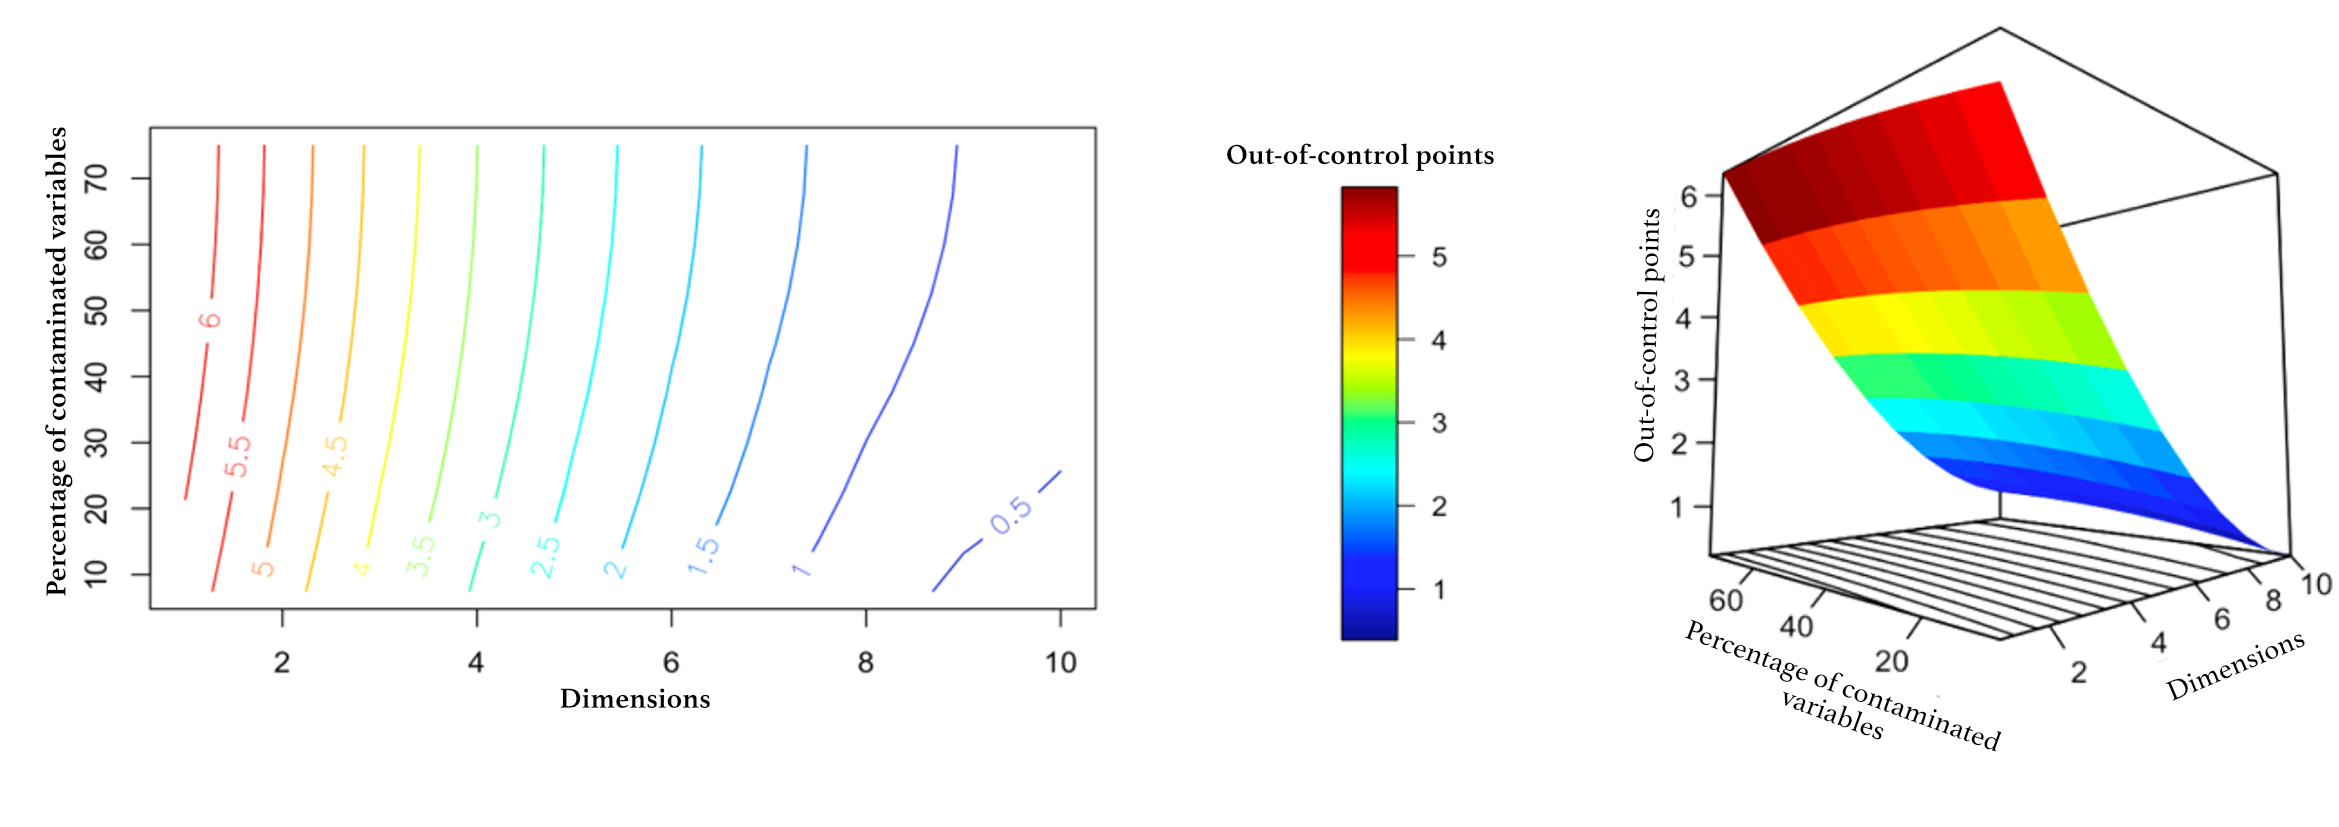
\includegraphics[width=0.9\linewidth,]{sensibilidadi} \end{center}

\caption{Contour plots and response surface obtained with the T2Qv chart.}
\label{fig:sensibilidad}
\end{figure}

The sensitivity analysis uses contour plots and response surfaces
(figure \ref{fig:sensibilidad}) to represent the number of
out-of-control points, considering the percentage of contaminated
variables in the \(k_i\) table and the number of dimensions represented.
The test data used in the model are recorded in 10 tables, each of which
includes 10 variables and each variable has three categories: High,
Medium, and Low. Table 10 (or table \emph{j}) has a different
distribution from the others, this being the contaminated table.

It is observed that the model is capable of identifying an
out-of-control point when working with \(p\) - 1 dimensions (9), even
with a low percentage of contaminated variables. When the number of
dimensions decreases to \(p\) - 2 (8) and the percentage of contaminated
variables is close to 100\%, it correctly detects 1 out-of-control
point. It is also observed that when the number of dimensions is lower,
stability is lost and the power of the test is reduced. Consequently,
the sensitivity analysis confirms that the T2Qv control chart performs
well when working with high dimensions.

\hypertarget{discusiuxf3n}{%
\section{Discusión}\label{discusiuxf3n}}

In statistical process control, there are still not many published
proposals for control charts for qualitative variables. Differences
between procedures for determining statistics and control charts in this
field make comparison difficult.

The T2Qv control chart, presented in this article, applies MCA, a
multivariate analysis technique that identifies latent structures
underlying the set of qualitative data and involves dimension reduction.
Therefore, from the outset, a data table with \(p\) dichotomous or
polytomous variables (\(p\) \textgreater{} 3) is required. It is worth
remembering that the sensitivity analysis determined that this proposal
performs well when working with high dimensions and loses stability at
low dimensions. Thus, while in the example with simulated data
\emph{Datak10Contaminated} presented in this research, the T2Qv analyzes
the behavior of 10 variables, in several reviewed studies, the
application cases analyze only two or three, which would lead to the
application of a simple correspondence analysis, not multiple.
Therefore, these cases could not be treated with the T2Qv.

Examples include the Optimal Linear Combination of Poisson Variables for
Multivariate SPC, by \citet{epprecht2013optimal}, whose registered
application case in their publication analyzes two variables related to
the count of defects in the production of ceramic jars. The GMDS chart
by \citet{raza2019design} was exemplified with a telecommunications
dataset taken from \citet{jiang2002process}, consisting of only two
variables. The multivariate control chart developed by
\citet{pastuizaca2015multivariate}) for \emph{p} correlated quality
attributes applies fuzzy theory and analyzes two tables taken from
publications by \citet{taleb2009control} and
\citet{taleb2006multivariate}, the first with three variables related to
frozen food, and the second with three variables on porcelain
production.

Another feature of the T2Qv chart is that each sample is a group
composed of a set of individuals, a table. The example of simulated data
\emph{Datak10Contaminated} includes a set of 10 tables and 11 variables,
each table is a sample, consisting of 100 observations and is
represented as a point in the Hotelling's T2 chart.

In publications by several authors, it can be observed that in their
application examples, only one table is analyzed, with dimensions
\emph{n} (rows) x \emph{p} (variables), where each row \(n_i\) is a
sample. For instance, the MNP control chart by \citet{lu1998control}
contains a simulated data table of 30 samples in their article, where
each sample is a single object that records the count of defects for
three quality characteristics. Similarly, \citet{chiu2007} presented an
exemplification of their MP control chart using a simulated data table
of 26 samples, where each sample represents an object that records the
\emph{D} number of defects or non-conformities associated with three
quality characteristics.

In the T2Qv control chart presented in this article, each of the
individuals (rows) that make up the different samples can have different
configurations depending on the categories of the variables.

On the other hand, other authors who have investigated multivariate
control charts for attribute data, although they consider several
quality characteristics in their analysis, ultimately classify each
individual by only one of the analyzed variables. This is the case with
\citet{ranjan2008multivariate}, whose proposal is demonstrated with an
application case that controls 7 quality characteristics in 24 samples
whose size varies between 20 and 404 individuals. The variables
correspond to 6 types of paint defects on the cover of ceiling fans:
poor coverage, overflow, puckering defect, bubbles, paint defects, and
polishing defects. The seventh characteristic is the absence of defects.
Each individual is classified by their most predominant defect;
therefore, only one type of defect or absence of defects appears in
their record, resulting in a loss of information about the combined
effect of the variables on the process.

Control charts that incorporate multivariate techniques are applied to
the analysis of categorical and numerical variables in the same data
table. For example, the PCA Mix control chart \citep{Ahsan2020} converts
attribute variables into dummy variables and treats them together with
continuous variables to generate a kernel matrix and calculate the
principal components. One weakness of this proposal is that its
performance decreases in the presence of extremely imbalanced
proportions of qualitative variable categories, a situation that is
proposed to be corrected by applying the Kernel PCA (KPCA) method, a
non-linear version of the conventional PCA that models non-Gaussian
distributions.

These performance adjustments correspond to a phase II of control
charts, with a view to their optimization. The T2Qv is a multivariate
process control chart that handles qualitative variables in phase I;
therefore, its efficiency evaluation has not yet been considered, so
both charts are not comparable. However, it is precisely the change in
the distribution of the variable categories, from balanced to
imbalanced, or vice versa, that the T2Qv detects as an out-of-control
point.

An interesting proposal is that of \citet{Saltos2020}, who use the
concept of depth for analyzing a data table in the field of education,
but ultimately, the representation of academic performance is univariate
and carried out using an r control chart. The ACM, being a factorial
technique that works in terms of variability association, causes
information common to all or the vast majority of cases to be stable and
therefore not appear on the primary axes, at best it is concentrated at
the graph's origin. In fact, in the T2Qv application, when a category of
a variable is constant in a table of the database, an error is reported
that prevents execution, but if there is at least one different case, it
would be represented as a point far away at some extreme of the graph,
while the category with the highest frequency would be located as a
point at the center. This could be a characteristic of the nature of the
ACM, which can only partially represent the variability of information
in its two dimensions.

To correct this problem, the methodology proposed in this research, in
conjunction with the ACM technique, uses the T2Qv chart which, as
established in the sensitivity analysis, works best with the highest
number of dimensions, i.e., collects the most variability to identify
the out-of-control point (the point table). Additionally, a subsequent
comparative analysis establishes the \(\chi^{2}\) distance between the
values reported by the categories of the concatenated table and the
point table for a specific variable and represents it in a bar chart,
which allows the identification of the variables that are producing the
most anomalies. Finally, the application facilitates the comparison of
the distribution of categories of the variable analyzed in the point
table and the concatenated table through an interactive graphical
resource that uses pie charts.

An opportunity for future research related to multivariate control for
qualitative variables could be the optimization of the graph, with a
control limit that adjusts to the specific parameters of the analysis,
taking it to a phase II of statistical process control. Another
opportunity would be the development of a methodology that goes beyond
the analysis of the first latent dimension, which is what the proposal
of this research does when applying ACM. The incorporation of a Meta
Biplot \citep{galindojk}, for example, could be viable, a technique that
cross-analyzes all latent dimensions.

\hypertarget{conclusions}{%
\section{Conclusions}\label{conclusions}}

This article presents a tool for multivariate statistical process
control that performs analysis of qualitative data, which is called the
T2Qv control chart, based on Multiple Correspondence Analysis.
Normalized coordinates are represented by the robust Hotelling T2 chart.

To facilitate the dissemination and application of the proposed method,
a reproducible statistical package has been developed in R, called T2Qv
and available on CRAN, which allows for the visualization of results in
a flat or interactive manner, and includes a Shiny panel that contains
all integrated functions in the same space.

This proposal generates a graph of the MCA of the concatenated table,
which serves as a reference for comparing other MCA graphs of tables
that have been identified as out-of-control points on the Hotelling
chart. This allows verification of which variable categories have had
changes in their location in both graphs, which may be causing changes
in the centrality of the process and causing it to be out of control.

To facilitate interpretation of the behavior of the variables, a
chi-squared distance analysis is performed between the categories of the
concatenated table and those of the tables reported as out of control,
analytically and graphically, including interactive graphics that
present the percentage distribution of the analyzed variable categories.

In a multivariate context, all variables contribute to a greater or
lesser extent to explaining the behavior of the process, so that
out-of-control output cannot be attributed to the individual action of a
variable or to the separate action of a group of them, but rather to the
combined effect of correlated variables. Therefore, a multivariate
approach is necessary in statistical process control.

The sensitivity analysis determined that the T2Qv control chart has good
performance when working with high dimensions, but loses stability at
low dimensions.

There are not many published proposals for multivariate statistical
process control for qualitative variables. The differences between
procedures for determining statistics and control charts in this field
make comparison difficult.

The T2Qv control chart addresses the need for a multivariate control
chart for qualitative variables in social processes, where the use of
nominal and ordinal variables is very common.

% %%%%%%%%%%%%%%%%%%%%%%%%%%%%%%%%%%%%%%%%%%
% %% optional
% \supplementary{The following are available online at www.mdpi.com/link, Figure S1: title, Table S1: title, Video S1: title.}
%
% % Only for the journal Methods and Protocols:
% % If you wish to submit a video article, please do so with any other supplementary material.
% % \supplementary{The following are available at www.mdpi.com/link: Figure S1: title, Table S1: title, Video S1: title. A supporting video article is available at doi: link.}

\vspace{6pt}

%%%%%%%%%%%%%%%%%%%%%%%%%%%%%%%%%%%%%%%%%%

%%%%%%%%%%%%%%%%%%%%%%%%%%%%%%%%%%%%%%%%%%

%%%%%%%%%%%%%%%%%%%%%%%%%%%%%%%%%%%%%%%%%%

%%%%%%%%%%%%%%%%%%%%%%%%%%%%%%%%%%%%%%%%%%
%% optional


%%%%%%%%%%%%%%%%%%%%%%%%%%%%%%%%%%%%%%%%%%
% Citations and References in Supplementary files are permitted provided that they also appear in the reference list here.

%=====================================
% References, variant A: internal bibliography
%=====================================
%\reftitle{References}
%\begin{thebibliography}{999}
% Reference 1
%\bibitem[Author1(year)]{ref-journal}
%Author1, T. The title of the cited article. {\em Journal Abbreviation} {\bf 2008}, {\em 10}, 142--149.
% Reference 2
%\bibitem[Author2(year)]{ref-book}
%Author2, L. The title of the cited contribution. In {\em The Book Title}; Editor1, F., Editor2, A., Eds.; Publishing House: City, Country, 2007; pp. 32--58.
%\end{thebibliography}

% The following MDPI journals use author-date citation: Arts, Econometrics, Economies, Genealogy, Humanities, IJFS, JRFM, Laws, Religions, Risks, Social Sciences. For those journals, please follow the formatting guidelines on http://www.mdpi.com/authors/references
% To cite two works by the same author: \citeauthor{ref-journal-1a} (\citeyear{ref-journal-1a}, \citeyear{ref-journal-1b}). This produces: Whittaker (1967, 1975)
% To cite two works by the same author with specific pages: \citeauthor{ref-journal-3a} (\citeyear{ref-journal-3a}, p. 328; \citeyear{ref-journal-3b}, p.475). This produces: Wong (1999, p. 328; 2000, p. 475)

%=====================================
% References, variant B: external bibliography
%=====================================
\reftitle{References}
\externalbibliography{yes}
\bibliography{mybibfile.bib}

%%%%%%%%%%%%%%%%%%%%%%%%%%%%%%%%%%%%%%%%%%
%% optional

%% for journal Sci
%\reviewreports{\\
%Reviewer 1 comments and authors’ response\\
%Reviewer 2 comments and authors’ response\\
%Reviewer 3 comments and authors’ response
%}

%%%%%%%%%%%%%%%%%%%%%%%%%%%%%%%%%%%%%%%%%%
\end{document}
